\documentclass{article}
%\documentclass{cernrep}
\usepackage{hyperref}
\usepackage{lineno}
%\linenumbers
\usepackage{a4}
\usepackage{epsfig}
\usepackage{lineno,url}
\usepackage{listings}
\usepackage{amsthm}
\newtheorem{exercise}{Exercise}
%\usepackage{color}
\usepackage{tcolorbox}
\usepackage{lipsum}
\tcbuselibrary{skins,breakable}
\usetikzlibrary{shadings,shadows}
\renewcommand{\familydefault}{\sfdefault}

\definecolor{codegreen}{rgb}{0,0.6,0}
\definecolor{codegray}{rgb}{0.5,0.5,0.5}
\definecolor{codepurple}{rgb}{0.58,0,0.82}
\definecolor{backcolour}{rgb}{0.95,0.95,0.92}
\newcommand{\magenta}[1]{\textcolor{magenta}{#1}}

\lstdefinestyle{mystyle}{
    backgroundcolor=\color{backcolour},   
    commentstyle=\color{codegreen},
    keywordstyle=\color{magenta},
    numberstyle=\tiny\color{codegray},
    stringstyle=\color{codepurple},
    basicstyle=\footnotesize,
    breakatwhitespace=false,         
    breaklines=true,                 
    captionpos=b,                    
    keepspaces=true,                 
    numbers=left,                    
    numbersep=5pt,                  
    showspaces=false,                
    showstringspaces=false,
    showtabs=false,                  
    tabsize=2,
    basicstyle=\ttfamily\footnotesize
}

\newenvironment{block}[1]{\tcolorbox[beamer,%
    noparskip,breakable,
    colback=backcolour,colframe=blue,%
    colbacklower=backcolour!75!backcolour,%
    title=#1]
    }%
    {\endtcolorbox}

 
\lstset{style=mystyle}
%\textheight 22cm
%%%%%%%%%%%%%%%%%%%%%%%%%%%%%%%%%%%%%%%%%%%%%%%%%%%%%%%%%%%%%%%%%%%%%%%
\newcommand\eps{\varepsilon}
\newcommand\erf{\mathop{\mathrm{erf}}}
\newcommand\pt{\partial}
%%%%%%%%%%%%%%%%%%%%%%%%%%%%%%%%%%%%%%%%%%%%%%%%%%%%%%%%%%%%%%%%%%%%

\newcounter{myexercise} 
\newcommand\showex{\stepcounter{myexercise}\themyexercise}

\usepackage{geometry}
 \geometry{
 a4paper,
 total={160mm,240mm},
 left=25mm,
 top=30mm,
 }
\begin{document}
%\linenumbers
\title{Transverse Linear Beam Dynamics\\ Primer using Python}
\author{ G. Sterbini, A. Latina, A. Poyet, CERN \\
V. Ziemann, Uppsala University}
\date{\today}
\maketitle
%%%%%%%%%%%%%%%%%%%%%%%%%%%%%%%%%%%%%%%%%%%%%%%%%%%%%%%%%%%%%%%%%%%%%%%
% \begin{abstract}\noindent
% bla
% \end{abstract}
%
%%%%%%%%%%%%%%%%%%%%%%%%%%%%%%%%%%%%%%%%%%%%%%%%%%%%%%%%%%%%%%%%%%%%%%%
%

\section{Introduction}
%
The purpose of this document is to complement with hands-on numerical exercises the CAS lectures on Transverse Linear Beam Dynamics. 
The numerical calculations will be illustrated with the help of the Python~\cite{PYTHON} general-purpose programming language\footnote{The reader can also use Octave \cite{OCTAVE} or MATLAB~\cite{MATLAB} to solve similar problems.}. The 
reader be asked to ``play around'' with the software and then
use it to solve simple beam optics problems.

This Chapter will introduce the
basic concepts and the software framework and will help to maximize the benefit drawn from the tutorial 
sessions at CAS. We start by introducing some basic theoretical concepts first, but illustrate the
ideas with, often trivial, examples in Python as we go along. Exercises are 
interspersed in the text and readers are 
encouraged to solve them. We will discuss the solutions at during the hands-on sessions at CAS. 
\par
This document focuses on Python, loosely following~\cite{VZAPB}, and its heavily based on the Octave/MATLAB version of this report~\cite{TUTOCT}. Most examples in the first part
of this tutorial are addressing the single particle motion.
\vspace{3mm}
\begin{block}{Disclaimer}
\begin{itemize}
    \item These exercises address the absolute newcomer in the field and the level is adapted accordingly. The exercises will help to visualize the concepts and provide an introduction to the basic numerical approach.
    \item In this hands-on tutorials we will use Python 3.8 and we assume the reader has some basic knowledge of Python.
\end{itemize}
\end{block}

%
\section{Ray tracing}
%
The motion of charged particles with respect to the ``center of the beam pipe'' in
an accelerator conceptually resembles the motion of optical rays with respect 
to the optical axis. In the latter case, a ray at a given longitudinal position 
$s$ is characterized by its distance
$x$ and its angle $x'$ with respect to the optical axis. In the absence of 
lenses or prisms, the light ray moves on a straight line. Its distance to the optical axis $\hat x$ at
a downstream location $\hat s$ therefore changes according to $\hat x=x+Lx',$
where we assume that $L$ is the distance between $s,$ where the ray's
coordinates are $(x, x'),$ and $\hat s,$ where the coordinates are $(\hat x, \hat x').$ 
Since it moves on a straight line, the angle does not change from $s$ to 
$\hat s,$ such that we have $\hat x'=x'.$ The two equations for $\hat x$ 
and $\hat x'$ can be combined in a single equation,
\begin{equation}\label{eq:drift}
\left(\begin{array}{c} \hat  x\\ \hat x'\end{array}\right)
=\underbrace{\left(\begin{array}{cc} 1 &L\\ 0 & 1\end{array}\right)}_{D}
\left(\begin{array}{c} x\\x'\end{array}\right)\ ,
\end{equation}
where the motion from $s$ to $\hat s$ is encapsulated in the matrix. 

\begin{exercise}
Show that multiplying two $D$ matrices, one with $L_1$ and the other with $L_2$ in the upper right corner, produces a $D$ matrix with the sum of the distances in the upper right corner.
\end{exercise}

When a ray passes a focusing (thin) lens, its angle $x'$ changes proportionally
to the transverse distance $x$ of the ray from the center of the lens, which we assume 
to be aligned with the optical axis. Recall the definition of the {\em focal length}, which 
requires a lens to deflect all parallel rays, independently of their transverse position,
in such a way, that the rays cross the optical axis at the same point -- the focal
point. This point is located at a distance $f$, the {\em focal length}, downstream of the lens.
We therefore require that the change of angle in the lens is given by $\hat x'=x'-x/f.$
Since we assumed the lens to be very thin, the transverse position of the ray does
not change and we have $\hat x=x.$ Here we assumed that the coordinates of the rays,
immediately upstream of the lens are $(x,x')$ and immediately downstream they
are $(\hat x, \hat x').$ Note that also these two equations can be combined into 
the following matrix-valued equation
\begin{equation}\label{eq:quad}
\left(\begin{array}{c} \hat x\\ \hat x'\end{array}\right)
=\underbrace{\left(\begin{array}{cc} 1 &0\\ -1/f & 1\end{array}\right)}_{Q}
\left(\begin{array}{c} x\\x'\end{array}\right)\ ,
\end{equation}
where a $f>0$ describes a focusing lens and $f<0$ a defocusing lens.

\begin{exercise}
How do you describe a ray that is parallel to the optical axis?
\end{exercise}

\begin{exercise}
How do you describe a ray that is on the optical axis?
\end{exercise}

\begin{exercise}
\label{ex4}
Show that, by multiplying the respective matrices,  a parallel ray, which first passes through a lens with focal length $f$ and then moves on a straight line, actually crosses the optical axis at a distance $L=f$ downstream of the lens. 
\textbf{Hint}: think a little extra about the correct order of the matrices.
\end{exercise}

A preliminary analysis of optical systems can easily be described by the matrices,
they are called Ray -- or ABCD-matrices in the optics literature~\cite{SIEGMAN}. But
optics is not exactly our topic, and we will therefore turn to charged particles,
instead.
\par
As a matter of fact, we can describe the linear motion of charged particles in the 
presence of magnetic lenses by the same mathematical framework, namely with
matrices; in accelerator physics they are usually referred to as {\em transfer matrices.}
We only have to establish a few correspondences beforehand. For charged particles, 
the optical axis can be visualized as the center of the beam pipe. Moreover, as already mentioned, at a 
longitudinal position $s,$ a particle can also be characterized by its distance 
$x$ and and angle $x'$ with respect to the center of the beam pipe. Here, we need
to point out that for charged particles this description is valid under the approximation of moderately 
small angles $x',$ which is referred as the {\em paraxial approximation} and is valid 
for angles in the range of a few tens of mrad. But this is usually valid in
accelerators -- 10\,mrad correspond to a change of distance of 10\,mm per meter!
\par
In the absence of external influences -- this can be visualized as a piece of beam 
pipe without magnets -- charged particles also move on a straight line. The matrix 
that maps the position $x$ and the angle $x'$ from one end of the empty pipe to the other 
end is the same we used for light rays and is given in Equation~\ref{eq:drift}. 
This matrix is commonly referred to as the {\em matrix for a drift space} as the 
empty piece of beam pipe is referred to as a {\em drift space}. 
\par
The elements corresponding to the optical lenses are magnetic elements with a 
magnetic field that depends linearly -- in linear optics  -- on the transverse position $x$. Note the
resemblance with the light rays: all parallel rays have to go through the focal
point downstream and that requires that the deflection angle of each ray has to
be proportional to its distance from the optical axis. In the same way charged particles are deflected more, due to the Lorentz force that the moving 
particles experience, if they are further from the axis of the magnet. Magnets with 
the required linearly rising magnetic field are {\em quadrupoles} and, if they are
moderately short with respect to its focal length $f$, they can be described by the matrix in Equation~\ref{eq:quad}.
Their inverse focal length $1/f$ is directly proportional to the magnetic gradient 
$\pt B_y/\pt x$, but we leave the details of the conversion to more advanced 
texts~\cite{VZAPB,WOLSKI,WIEDEMANN,SYLEE}.
% their length $l,$ which is assumed to be short, and their momentum $p$ through 
% $1/f=(\pt B_y/\pt x)l/(p/e),$ where $e$ is the electric charge of the particles.
\par
We note, however, that the magnetic fields in the quadrupoles have to fulfill
Maxwell's equations. This forces the transverse components $B_x$ and $B_y$ of 
the magnetic field to obey the curl equation: $\pt B_y/\pt x - \pt B_x/\pt y =0.$ 
A linearly increasing field component in one direction causes the other component 
to decrease. Quadrupoles therefore focus particles in one transverse plane, but 
defocus the same particles in the other plane. Since we will only consider one 
plane in this first part of the tutorial, we will not encounter this ``feature'' directly. We will, 
however, build beamlines consisting of both focusing and defocusing quadrupoles. 
The motivation to use both types of quadrupoles is to be able to describe the other
plane of the accelerator as well.
\par
There are many more magnets that are used to guide the beam -- big dipoles and small
steering magnets -- and other magnets to correct various effects, but we will, in
the early sections of this tutorial, confine ourselves to drift spaces and quadrupoles 
and will build larger beam optical systems with these elements alone. We will 
implement most matrix manipulations in software in order to avoid excessive matrix 
calculations by hand.
%
\section{A simple code to transport particles}

In the following we are going to introduce a simple code for transporting particles in a beamline using Python. The code is deliberately kept simple in order to make its
structure transparent, sometimes at the expense of its overall
performance.

\subsection{The element: a matrix representation}

Finally our task is to follow a particle through a sequence of drift spaces and quadrupoles (elements),
described by the matrices from Equation~\ref{eq:drift} and~\ref{eq:quad}.

To do so, we first encode the matrices in a convenient way by using functions, e.g.,
\begin{lstlisting}[language=Python]
import numpy as np
def D(L):
    '''Returns the matrix of a L-long drift'''
    return np.array([[1, L],[0, 1]])
\end{lstlisting}
The commands above define a function {\tt D($\cdot$)} that receives the length {\tt L} as input and 
returns the corresponding drift matrix from Equation~\ref{eq:drift}.
Likewise, we define the function
\begin{lstlisting}[language=Python]
def Q(f):
    '''Returns the matrix of a quadrupole with focal length f'''
    return np.array([[1, 0],[-1/f, 1]])
\end{lstlisting}
which returns the matrix from Equation~\ref{eq:quad}.

\subsection{Combining several elements: the beamline}

By combining drifts an quadrupoles we can define a beamline. We can think a beamline as a new element and associate to it an ``equivalent'' matrix obtained by the multiplication of the matrices of its elements.
\vspace{3mm} 
\begin{block}{Nota Bene}
In Python 3, the operator for matrix multiplication is the `@` operator.
\end{block}

For example, let us assume to have a sequence of a drift of 2.5 m followed by a quadrupole with a focal length of 3 m and a final drift of drift of 1.2 m. The equivalent matrix, $M$, of the combination of these elements is: 
\begin{lstlisting}[language=Python]
# Multiplication of matrices
M = D(1.2) @ Q(3) @ D(2.5)
\end{lstlisting}

\begin{block}{Nota Bene}
Please note the ordering of the matrices. Since we are considering to right-multiply our matrices with the particle vector ($x$,$x'$), the elements matrices should be ordered from the right to the left.
\end{block}

A natural way to define the beamline is to consider it as a list of elements.
\begin{lstlisting}[language=Python]
mybeamline = [D(2.5), Q(3), D(1.2)]
\end{lstlisting}

This has the advantage to use the `+' and `*' operation to combine beamlines as in the following example

\begin{lstlisting}[language=Python]
# two simple beamlines
mybeamline_1 = [D(2.5), Q(3), D(1.2)]
mybeamline_2 = [D(2), Q(-1)]
# building a third beamline using the list algebra of python
mybeamline_3 = (mybeamline_1*2+mybeamline_2)*3
\end{lstlisting}

Then we can compute the equivalent matrix of the beamline.

\begin{lstlisting}[language=Python]
def getEquivalentElement(beamline):
    '''Returns the equivalent single element of a beamline.'''
    # np.eye(2) gives the 2x2 identity matrix
    equivalentElement = np.eye(2)
    # NB: we reverse the order of the beamline ([ -1:: -1])
    for elements in beamline[-1::-1]:
        equivalentElement = equivalentElement @ elements
    return equivalentElement
\end{lstlisting}

In line 6 of the previous code block the {\rm [-1::-1]} expression is a trick to reverse the order of the element in the beamline (the last element will become the first one considered in the loop).

With the equivalent matrix we can therefore compute, given the initial position (x, x') of the particle at the entrance of the beamline, its position at the end.
\begin{lstlisting}[language=Python]
# initial position of the particle
x_start = [[0.2],[.3]]
# final position of the particle
x_end = getEquivalentElement(mybeamline_3) @ x_start
\end{lstlisting}

The above approach has at least one limit: we cannot resolve the position of the particle ``inside'' the beamline but only at its end.

To overcome this limitation, we can build a tracking engine that allows us to track the particle for all the elements in a beamline. For instance we can define 

\begin{lstlisting}[language=Python]
def transportParticles(x0, beamline):
    '''Returns the list of position in the beamline 
    starting from x0.'''
    x = [x0]
    for elements in beamline:
        x.append(elements @ x[-1])
    return np.array(x).transpose()[0]
\end{lstlisting}
and then
\begin{lstlisting}[language=Python]
transportParticles(x_start, mybeamline_3)
\end{lstlisting}



Still there is a problem: we are not able to associate to each element a corresponding $s$-position. We will overcome this limitation in the next Section.

\subsection{Tracking a particle along a beamline}
\label{sec:dict}

As presented, having an ``equivalent'' matrix allows to build complex elements starting from simpler ones. The drawback of this approach is that we lose the information of the particle position $s$ along the line.

In order to recover this flexibility we can define the elements as a dictionary having both the information of the matrix and the one relative to the elements length. For example

\begin{lstlisting}[language=Python]
def D(L):
    '''Returns the list of a L-long drift'''
    # NB: we return a list with a dict
    # the dict contains the matric (the transformation)
    # and the element length 
    return [{'matrix':np.array([[1, L],[0, 1]]), 'length':L}] 

def Q(f):
    '''Returns the list of a quadrupole with focal length f'''
    # NB: we return a list with a dict
    # the dict contains the matric (the transformation)
    # and the element length 
    return [{'matrix':np.array([[1, 0],[-1/f, 1]]), 'length':0}]
\end{lstlisting}
We can therefore redefine the \texttt{getEquivalentElement} and \texttt{transportParticles} methods accordingly.

\begin{lstlisting}[language=Python]
def getEquivalentElement(beamline):
    '''Returns the equivalent single element of a beamline'''
    # we start from an identity matrix (np.eye)
    # with the same dimension of the matrix of the
    # first element of the beamline
    equivalentElement = np.eye(beamline[0]['matrix'].shape[0])
    length = 0
    # NB: we reverse the order of the beamline ([-1::-1])
    for elements in beamline[-1::-1]:
        # we multiply the matrices 
        equivalentElement = equivalentElement @ elements['matrix']
        # and we add the lengths
        length = length + elements['length']
    # we return the dict with the "usual" keys (matrix and length)
    # as for the definition of the D and Q functions
    return {'matrix':equivalentElement, 'length':length}

def transportParticles(x0,beamline):
    '''Track the particle(s) x0 along the beamline'''
    coords = [x0]
    s = [0]
    for elements in beamline:
        coords.append(elements['matrix'] @ coords[-1])
        s.append(s[-1] + elements['length']) 
    coords = np.array(coords).transpose()
    return {'x':  coords[:,0,:],
            'px': coords[:,1,:],
            's':  np.array(s),
            'coords': coords,}
\end{lstlisting}
and then
\begin{lstlisting}[language=Python]
# NB: since each element is a list, we can concatenate 
# with the `+` and `*` operators.
mybeamline_1 = D(2.5) + Q(3) + D(1.2)
mybeamline_2 = D(2) + Q(-1)
# building a third beamline using the list algebra of python
mybeamline_3 = (mybeamline_1*2+mybeamline_2)*3
\end{lstlisting}



For convenience, we explicitly output the \texttt{x} and \texttt{px} parameters in the function \texttt{transportParticles}. In summary, using the simple approach shown above, we can

\begin{itemize}
    \item describe an element as a dictionary giving the information about linear matrix and element length,
    \item combine several elements in a list (beamline) and use a convenient algebra (`+' and `*') to concatenate and replicate different beamlines,
    \item reduce a beamline in a an equivalent element,
    \item track a particle along a beamline.
\end{itemize}

As example, we map the initial coordinates
 {\tt x\_start}, specified as a column vector, along the beamline and plot the 
transverse position {\tt x} as a  function of the longitudinal position $s$.
\begin{lstlisting}[language=Python]
import matplotlib.pyplot as plt
f=1
L=1/10

# NB: combination of list to prepare a generic beamline
beamline= 5*D(L)+Q(-f)+10*D(L)+Q(.84*f)+5*D(L)
x_start = [[0.002],[0]]
# We encourage to try other initial condition, e.g.
# x_start = [[0],[0]]

# NB: we concatenate 40 beamline
output=transportParticles(x_start,beamline*40)
# plotting the results

plt.plot(output['s'],output['x'][0]*1000,'o-b',lw=3)
plt.grid(True)
plt.xlabel('s [m]')
plt.ylabel('x [mm]')
\end{lstlisting}

The result of the above snippet of code is shown in Figures~\ref{fig:first_bl}-\ref{fig:second_bl}.
\begin{figure}
    \centering
    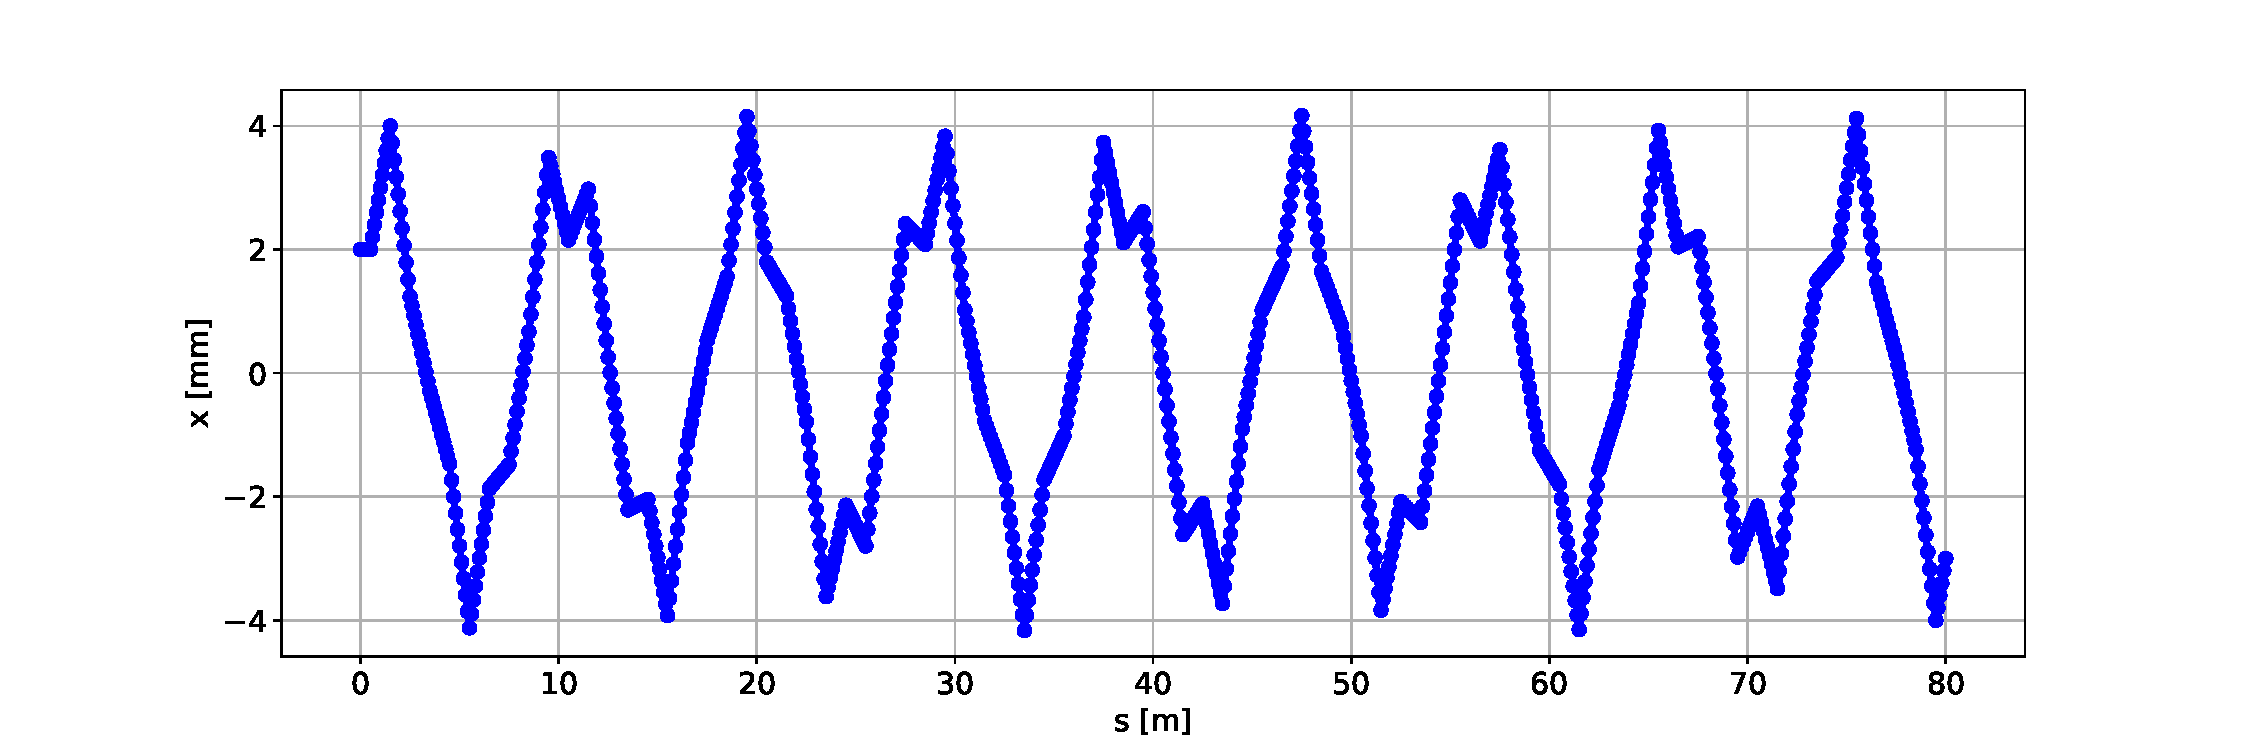
\includegraphics[width=1\textwidth]{_img_primer/first_bl.pdf}
    \caption{The x-position of our particle along the beamline.}
    \label{fig:first_bl}
\end{figure}
\begin{figure}
    \centering
    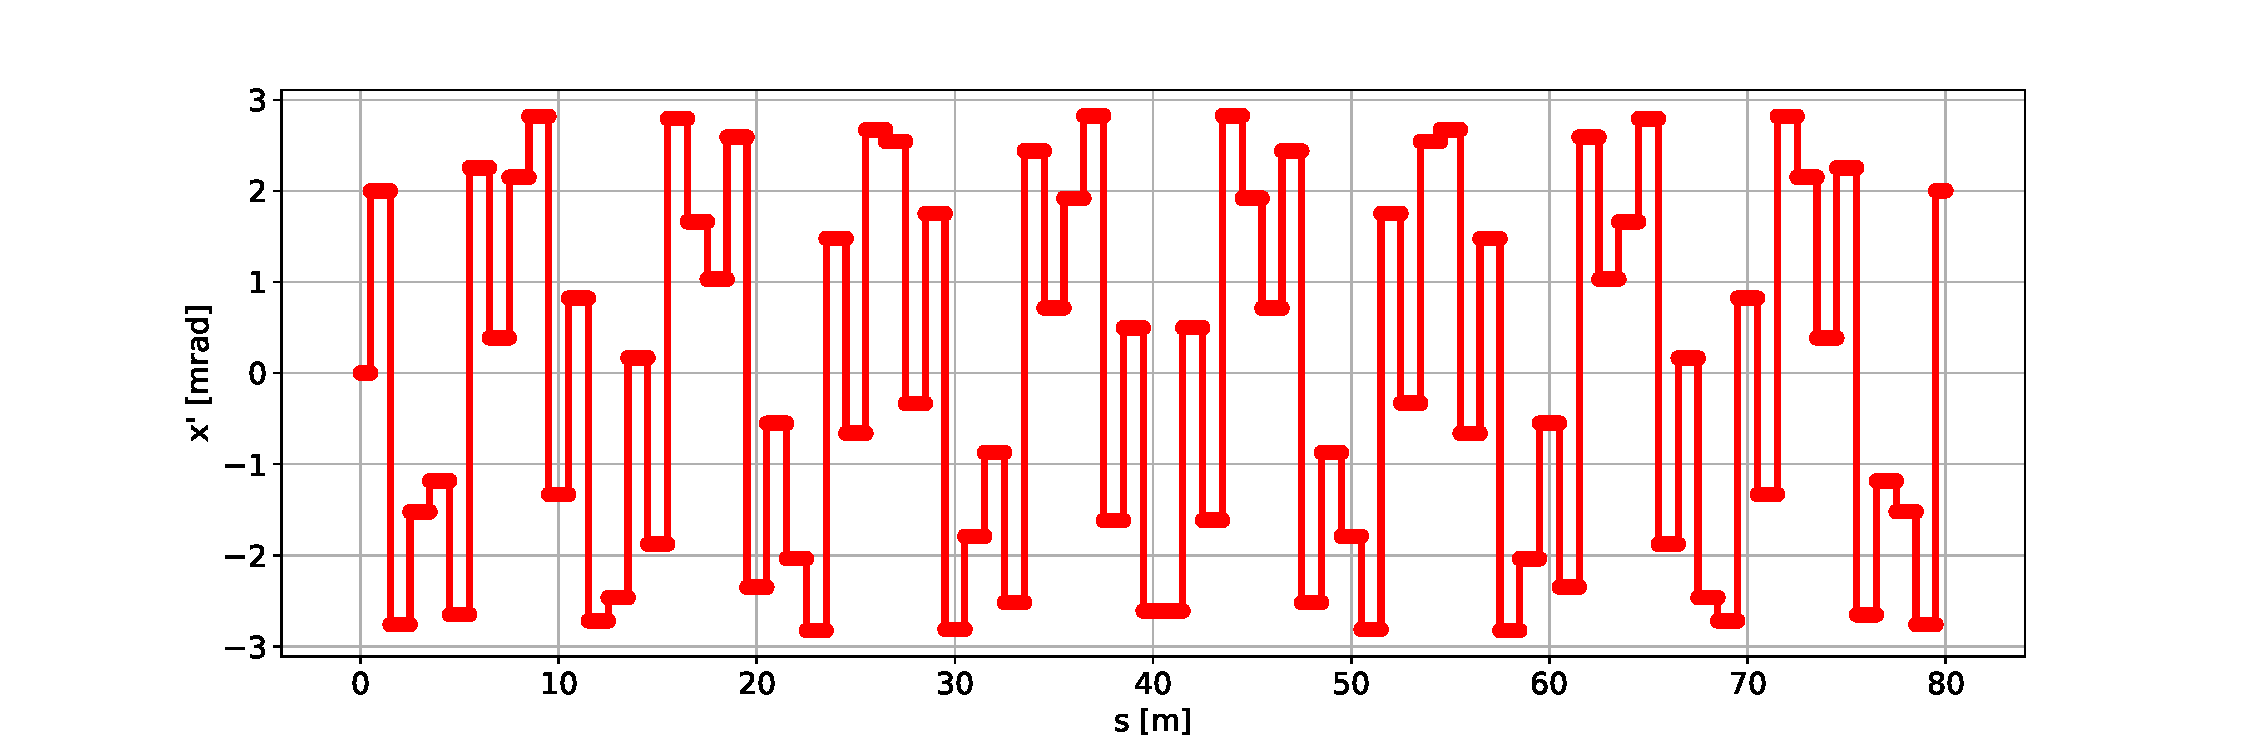
\includegraphics[width=1\textwidth]{_img_primer/second_bl.pdf}
    \caption{The x'-position of our particle along the beamline.}
    \label{fig:second_bl}
\end{figure}

We will see in the next exercises how to use those simple functions to put our hands-on the beam dynamics. A limited part of the exercises comes with some hints to suggest the direction of the solutions. The solutions are available in a separate document \cite{solutions}.


\begin{exercise}
 Set $F=3$ and numerically verify what you found in Exercise~\ref{ex4}, 
  namely that parallel rays cross the axis after a distance $L=F.$ 
  
  \textbf{Hint}: use, first, the \texttt{getEquivalentElement} and, then, the \texttt{transportParticles} functions, as defined in Section~\ref{sec:dict}, and show that the conclusion is the same.
\end{exercise}

\section{Studying simple beamlines}

There are notable beamlines frequently considered in synchrotrons, such as the FODO beamline (also known as FODO lattice):
\begin{lstlisting}[language=Python]
#the FODO beamline
f = 2.5
beamline = 5*D(0.1) + Q(f) + 10*D(0.1) + Q(-f) + 5*D(0.1)
\end{lstlisting}
The first line defines the focal length {\tt f} to be 2.5\,m and then defines
a list, that follows the conventions defined above. The beamline is composed summing 5 lists. 
The first list of the beamline describes 5 segments of a drift space, each being 0.1\,m long. The second 
list describes a thin quadrupole. The third list describes a drift space, consisting of ten 
segments with length 0.1\,m each. The fourth list
describes a second quadrupole, this time with a negative focal length. The last list is
equal to the first one. We call the list that describes our beamline {\tt FODO}, because 
it consists of an alternating sequence of focusing (F) and defocusing (D) quadrupoles,
separated by not-focusing (O) drift spaces. The arcs of the LHC collider or the SPS synchrotron are based on them. The reason to alternate the quadrupole
polarity is to focus in both transverse planes equally, despite  each quadrupole affects
the two planes in the opposite manner.
\begin{exercise}
Recall that the imaging equation for a lens is $1/b+1/g=1/f,$
  which corresponds to a system of one focusing lens with focal length $f,$ sandwiched
  between drift spaces with length $b$ and $g$, respectively. Write a beamline
  description that corresponds to this system. We will later return to it and analyze it. 
\end{exercise}
% Having a description of sequence of elements in a beamline available, we now will turn to
% assembling all matrices that map the coordinates of a particles at the start of the beam 
% line to each and every beamline element. This will allow us to follow a particle on
% its journey through the accelerator. 
% \par
% To do so we need to loop in the element of the beamline and for each element to compute the matrix multiplication with the corresponding matrix. A possible  implementation is the following:
% \begin{lstlisting}[language=Python]
% for element in beamline:
%     beamlist.append((element[0] @ beamlist[-1][0],beamlist[-1][1]+ element[1]))     
% \end{lstlisting}
% The previous code will append a new tuple to the beamlist for each element in the beamline. This new tuple will have, in the first position, the vector of the trace-space obtained as product of the matrix and the previous beamlist trace-space vector. Please note the in python3 we use the operator '@' for matrix multiplication and pay attention to the use of the indexes (in python the indexing starts with 0).
% The second element of the tuple is the incremental $s$-position along the beamline.

% From the beamlist we will be able to make plots with the horizontal axis denoting the 
% longitudinal position.

% Now we are ready to use this code. As example, we map the initial coordinates
% {\tt x0}, specified as a column vector, along the beamline and plot the 
% transverse position {\tt x} as a  function of the longitudinal position $s.$
% \begin{lstlisting}[language=Python]
% # The drift
% D = lambda L: [(np.array([[1, L],[0, 1]]), L)]
% # The thin quadrupole
% Q = lambda f: [(np.array([[1, 0],[-1/f, 1]]), 0)]
% # the beamline
% f=2.5
% L_2=1
% beamline= 5*D(L_2/2/5)+Q(f)+10*D(L_2/(10))+Q(-f)+5*D(L_2/2/5)
% # the beamlist
% beamlist=[(np.array([[0],[0.001]]),0)]
% # the tracking
% for element in beamline:
%     beamlist.append((element[0] @ beamlist[-1][0],beamlist[-1][1]+ element[1]))
% # plotting the results
% from matplotlib import pyplot as plt
% %matplotlib inline
% plt.plot([i[1] for i in beamlist],[i[0][0]*1000 for i in beamlist],'o-b',lw=3)
% plt.grid(True)
% plt.xlabel('s [m]')
% plt.ylabel('x [mm]')
% \end{lstlisting}
% %
% In the previous code snippet keep in mind the following aspects:
% \begin{enumerate}
%     \item the use of \textit{lambda} function
%     \item the list of tuples to define beamlines and beamlist,
%     \item the algebra of list used to build a beamline,
%     \item the '@' operator for matrix multiplication,
%     \item the list comprehension used to plot the beamlist.
% \end{enumerate}
%  Note that we multiply
% the contents of {\tt data} by $10^3$ in order to convert it to mm, which is also
% annotated in the axes labels.

\begin{exercise}
Prepare initial coordinates that describe a particle that is on the optical axis, but has an initial angle $x'$ and plot the position $x$ along the beamline.
\end{exercise}

\begin{exercise}
Plot the angle $x'$ along the beamline.
\end{exercise}

The code only shows the trajectory in a single FODO cell. If we want to display the
trajectory, for example, through five consecutive cells, we only have to replace the definition of the {\tt beamline} early in the script by
\begin{lstlisting}[language=Python]
beamline = 5*beamline
\end{lstlisting}

\begin{exercise}
Plot both the position $x$ and the angle $x'$ through five cells.
\end{exercise}

\begin{exercise}
Plot the position $x$ through 100 cells, play with different values of the focal length {\tt F} and explore whether you can make the oscillations grow.
\end{exercise}

\begin{exercise}
Use the beamline for the imaging system you prepared in Exercise~6 and launch a particle with $x_0=0$ and an angle of $x'_0=1\,$mrad at one end. Verify that this particle crosses the center of the beam pipe at the exit of the beamline, provided that $b,g,$ and $f$ satisfy the imaging equation that is shown in Exercise~6. 
\end{exercise}
Up to now we transported single particles through a beamline. But
a beam consists of more than a few particles and in the following section we will show how to describe such an ensembles of particles.
%
\section{Many particles, the beam}
%
Each of the many particles in a beam has its individual coordinates $(x,x').$ Under 
most circumstances are the positions $x$ and angles $x'$ distributed according to a normal (also referred as Gaussian) distribution. We create the coordinates of $N$ particles as a $2\times N$
array {\tt beam} that we fill with normally distributed random numbers with the 
help of the function {\tt randn()}. 

The approach is very similar to the one used for the single particle but in this case the beam will be represented by a $ 2\times$ {\tt N\_particles} matrix.
\begin{lstlisting}[language=Python]
N_particles = 1000
beam = np.random.randn(2, N_particles)
x0 = 0
xp0 = 1
sigx = 1 
sigxp = 0.5 
beam[0,:] = sigx*beam[0,:] + x0
beam[1,:] = sigxp*beam[1,:] + xp0
\end{lstlisting}
The random numbers returned by \texttt{np.random.randn} have a mean of zero and unit rms, such that we scale them by multiplying
the first coordinate by the rms beam size {\tt sigx} and the second coordinate by the rms 
angular divergence {\tt sigxp}.
We can also introduce the initial offsets {\tt x0} and {\tt xp0}, which are then the 
respective means of the distribution. We can now verify that the distribution has the 
desired properties by calculating the beam parameters via
\begin{lstlisting}[language=Python]
print(f'Beam mean x [mm]: {np.mean(beam[0,:])}')
print(f"Beam mean  x' [mrad]: {np.mean(beam[1,:])}")
print(f'Beam rms size[mm]: {np.std(beam[0,:])}')
print(f"Beam rms divergence [mrad]: {np.std(beam[1,:])}")
\end{lstlisting}
where {\tt beam[0,:]} and  {\tt beam[1,:]} refer to the first and second row of the matrix {\tt beam}, which 
contains the positions and angles of all particles. The built-in functions {\tt np.mean()} and 
{\tt np.std()} return the average and rms values of the distribution, respectively.
\begin{exercise}
Define an ensemble of 1000 particles with an arbitrary first order ({\tt x0}, {\tt xp0}) and second order momenta( {\tt sigx} and {\tt sigxp}).
Verify the angular divergence of the beam is the one set.
\end{exercise}
%..............................................
\begin{figure}[tb]
\begin{center}
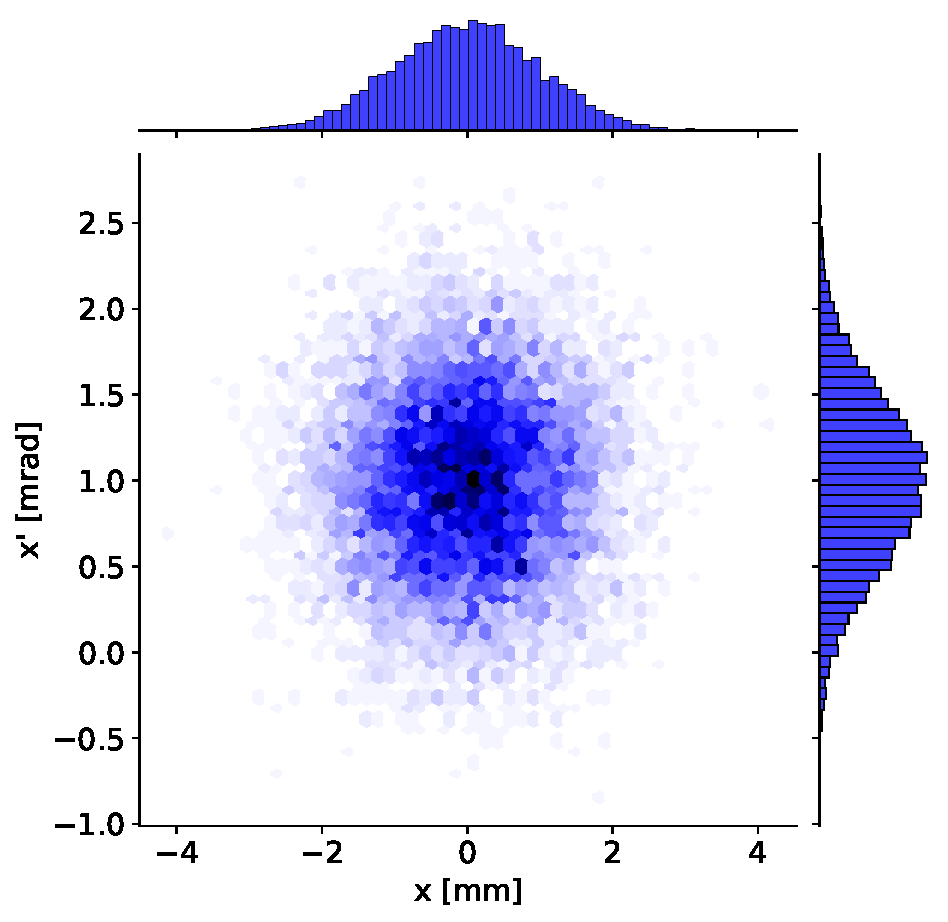
\includegraphics[width=0.47\textwidth]{_img_primer/before_drift.pdf}
\hskip 5mm
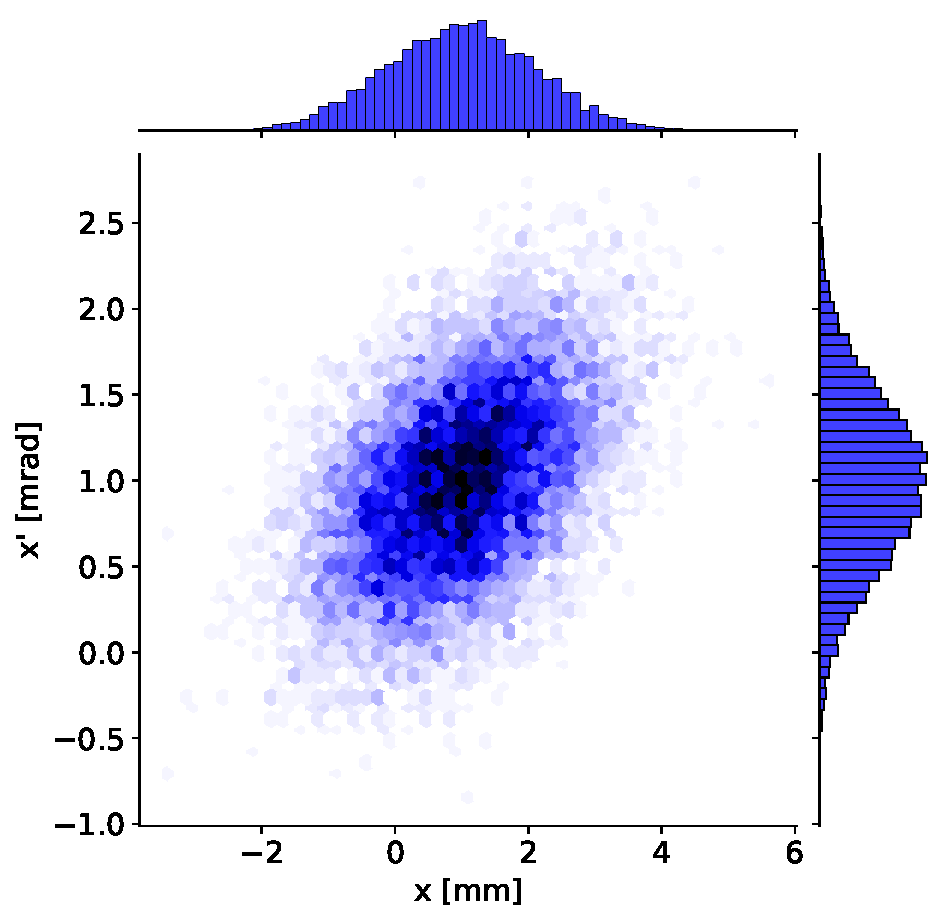
\includegraphics[width=0.47\textwidth]{_img_primer/after_drift.pdf}
\end{center}
\caption{\label{fig:beam}Particles at start (left) and after 1\,m drift space (right).}
\end{figure}
%..............................................
We can visualize the particle distribution by plotting one and two-dimensional 
histograms and contour plots. We can display the distribution using the \texttt{seaborn} plotting package, see left-side plot of Figure~\ref{fig:beam}.

\begin{lstlisting}[language=Python]
import seaborn as sns
g = sns.jointplot(x=beam[0,:], y=beam[1,:], kind="hex", color="b")
g.set_axis_labels("x [mm]", "x' [mrad]");
\end{lstlisting}

\par
We then use a transfer matrix {\tt R} to propagate the {\tt beam} to a downstream
location, here through a drift space with a length of 1\,m, by multiplying the {\tt beam}
with {\tt R} , as shown in the following example.
\begin{lstlisting}[language=Python]
beamAfterDrift = D(1)[0]['matrix'] @ np.array(beam)
\end{lstlisting}
Calling again  the {\tt seaborn} plotting function one gets the  right-hand side in 
Figure~\ref{fig:beam}. We find that the distribution has slightly changed shape:
the ellipse has rotated. Moreover, the mean of the horizontal distribution has 
changed to 1\,mm. This is a consequence of the initial angle $x'_0=1\,$mrad, which
caused the beam to move towards the positive x-axis by 1\,mm over the 1\,m long 
drift space. The horizontal width has increased to 1.1\,mm.
\par
Note that we specified the transverse dimensions and angle in mm and mrad instead
of m and rad. This is permissible, because transfer matrices describe a {\tt linear}
transformation, and multiplying the vector to the right by a factor, here $10^3,$
causes the output on the left of the matrix multiplication to be scaled by the same 
number.
\begin{exercise}
Transport the beam distribution of Exercise 12 in a drift of length 1 m. Compare the initial and final distribution.

Test of linearity.  Scale the input vector by 17 times the month of your birthday (85 if you are born in May) and verify that the output vector from the matrix multiplication has changed by the same factor.

Now launch 3 particles such that they define a triangle of surface A. Verify that this linear transport preserves the area of the triangle. 
\end{exercise}
\begin{block}{Nota Bene}
The `area preservation' property of the previous exercise is a very profound concept. In linear optics is related to the fact that the matrices we are considering are \href{https://en.wikipedia.org/wiki/Symplectic_matrix}{\textbf{symplectic}}\dots 
\end{block}


\par
%..............................................
\begin{figure}[tb]
\begin{center}
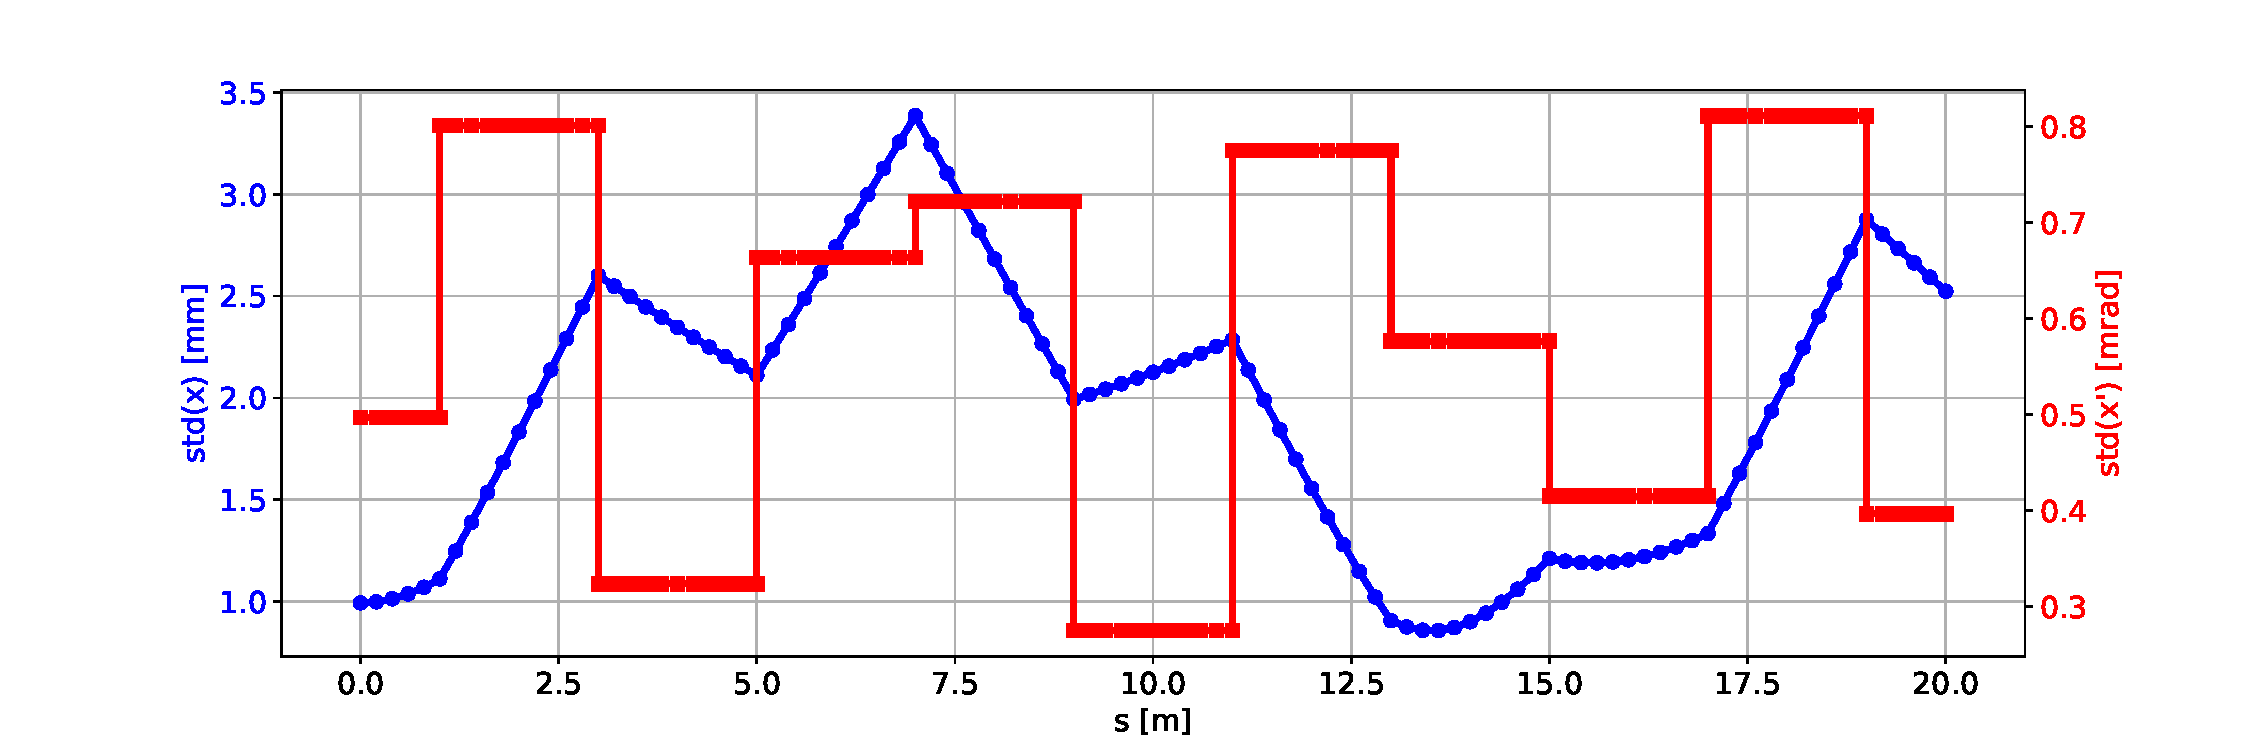
\includegraphics[width=\textwidth]{_img_primer/exercise14.pdf}
\end{center}
\caption{\label{fig:sigvzs}The beam size along the beamline made of five FODO cells.}
\end{figure}
%..............................................
We will continue to use mm and mrad for the transverse coordinates and will now 
calculate the beam size after every segment in the beamline. We use the previous approach 
to build a beamline of five consecutive FODO cells. Then we execute the following code:
\begin{lstlisting}[language=Python]
#prepare the optics
f = 2.5
L_2 = 2
fodo_lattice = 5*D(L_2/10)+Q(-f)+10*D(L_2/10)+Q(f)+5*D(L_2/10)

#prepare the beam
Npart = 10000
beam = np.random.randn(2, Npart)
x0 = 0
xp0 = 1
sigx = 1
sigxp = 0.5
beam[0,:] = sigx*beam[0,:]+x0
beam[1,:] = sigxp*beam[1,:]+xp0

output = transportParticles(beam, 5*fodo_lattice)

plt.plot(output['s'], np.std(output['x'],0), 'o-b', lw=3)
plt.grid(True)
plt.xlabel('s [m]')
plt.gca().set_ylabel('std(x) [mm]', color='b')
plt.gca().tick_params(axis='y', labelcolor='b')

ax2 = plt.gca().twinx()  # instantiate a second axes that shares the same x-axis
ax2.set_ylabel("std(x') [mrad]", color='r')
ax2.tick_params(axis='y', labelcolor='r')
plt.plot(output['s'], np.std(output['px'],0), 's-r', lw=3)
\end{lstlisting}
It is important to note that the approach of the previous code is identical to the one for single particle tracking. Indeed the {\tt beam} can represent a single particle or an ensemble of particle.
At the end of the script, we 
display the beam size as a function of $s$ and annotate the axes. Figure~\ref{fig:sigvzs}
shows the resulting plot. We observe that the beam size grows over the first meter, where
it traverses a defocusing quadrupole, which increases the beam size further until at 
$s=3\,$m. There the first focusing quadrupole reduces the beam size until the defocusing quadrupole 
at $s=5\,$m increases the beam size again, then the focusing quadrupole at $s=7\,$m 
reduces it again; and so forth. We also observe that the {\tt beam} initially defined with {\tt sigx}$=1\,$mm can become larger up to an rms beam size {\tt sigx}$>3\,$mm.

\begin{exercise}
Using the 5 FODO cells of Exercise 9, transport the beam of Exercise 13 and plot its rms size and divergence along the line.
\end{exercise}

\begin{exercise}
Starting from Exercise 14, what happens if you (a) increase or (b) reduce by a factor 2 the initial beam size and divergence ({\tt sigxp})?
\end{exercise}
Normally, one is not really interested in the histogram of the particle distribution.
Information about the centroid position, the beam size, and possibly the angular 
divergence are enough. So, wouldn't it be nice, 
if we could move the interesting quantities around, instead of thousands of sample
particles? It turns out that this is possible and that is the topic of the next section.
%
%%%%%%%%%%%%%%%%%%%%%%%%%%%%%%%%%%%%%%%%%%%%%%%%%%%%%%%%%
%
\section{Moving beams around}
%
To simplify the writing of many matrix-valued equations, we introduce the notation 
that the position $x$ is denoted by $x_1$ and the angle $x'$ by $x_2.$ This allows us
to express the propagation of the particle coordinates as $\hat x_i=\sum_{j=1}^2 R_{ij}x_j.$
If we have to deal with many particles we label them by a second subscript, separated from 
the first by a comma; $x_{2,17}$ is thus the angle of particle number~17.
\par
When we calculated the average beam position and angle using numpy functions, the software 
actually performed the following operations
\begin{equation}
X_1=\langle x_1\rangle = \frac{1}{N}\sum_{m=1}^N x_{1,m}
\qquad\mathrm{and}\qquad
X_2=\langle x_2\rangle = \frac{1}{N}\sum_{m=1}^N x_{2,m}\ ,
\end{equation}
where the index $m$ sums over the $N$ particles of the beam. The notation with the angle brackets 
denotes thus averaging over the ensemble of particles. We also introduced the quantities
$X_1$ and $X_2$ to denote the averages. Likewise, the rms quantities are calculated via
\begin{eqnarray}
\sigma_x^2&=& \sigma_{11}=\langle(x-X_1)^2\rangle = \frac{1}{N}\sum_{m=1}^N (x_{1,m}-X_1)^2\nonumber\\
\sigma_{x'}^2&=& \sigma_{22}=\langle(x'-X_2)^2\rangle = \frac{1}{N}\sum_{m=1}^N (x_{2,m}-X_2)^2\ .
\end{eqnarray}
By inspection, we should not be surprised that there is also a third variant of the above sums,
given by
\begin{equation}
\sigma_{12}=\langle(x-X_1)(x'-X_2)\rangle = \frac{1}{N}\sum_{m=1}^N (x_{1,m}-X_1)(x_{2,m}-X_2)\ ,
\end{equation}
which describes the correlation between position (index 1) and angle (index 2). This quantity
$\sigma_{12}$ is actually capable of describing the rotation of the contour in the right-hand
plot in Figure~\ref{fig:beam} that showed up after propagating the initial beam through
a 1\,m long drift space.
\par
These five quantities $X_1, X_2, \sigma_{11}, \sigma_{12},$ and $\sigma_{22}$ describe all 
the interesting properties of a beam. Note that $X_1$ and $X_2$ are the first moments of
the two-dimensional beam distribution and the $\sigma_{ij}$ with $i=1,2$ are the three 
independent second moments; actually they are the central moments, because they 
describe the second moments with respect to the centroids. Note that usually the
three independent second moments can be written to form a symmetric $2\times 2$--matrix
that is given by
\begin{equation}\label{eq:bmat}
\sigma=
\left(\begin{array}{cc} \sigma_{11} & \sigma_{12} \\ \sigma_{21}& \sigma_{22}\end{array}\right)\ ,
\end{equation}
with $\sigma_{21}=\sigma_{12}.$ We use the convention that sigmas without 
subscripts denote the matrix and sigmas with subscripts denote the matrix elements. 
We also point out that the sigma matrix changes from one location $s$ in the beamline 
to another location $\hat s.$ Remember that Figure~\ref{fig:sigvzs} shows the beam size
$\sigma_x=\sqrt{\sigma_{11}}$ as a function of $s$ along the beamline.
\par
In the more advanced literature~\cite{VZAPB,WOLSKI}, but also in Appendix~\ref{sec:propmom}, 
it is shown that the first and second moments propagate according to 
\begin{equation}\label{eq:prop}
\vec X(s_2) =  R\, \vec X(s_1)
\qquad\mathrm{and}\qquad
\sigma(s_2) = R\, \sigma(s_1)\, R^t\, ,
\end{equation}
where $\vec X(s)$ denotes the column vector with entries $X_1$ and $X_2$ at longitudinal
location $s.$ The first equation describes the remarkable fact that the centroid of
the beam -- the first moments -- propagate in the same way as single particles. The
second equation describes the propagation of the beam matrix, as defined in 
Equation~\ref{eq:bmat}. In Equation~\ref{eq:prop} we use the common convention to
denote the transpose of the matrix $R$ by $R^t.$
\par
%..............................................
\begin{figure}[tb]
\begin{center}
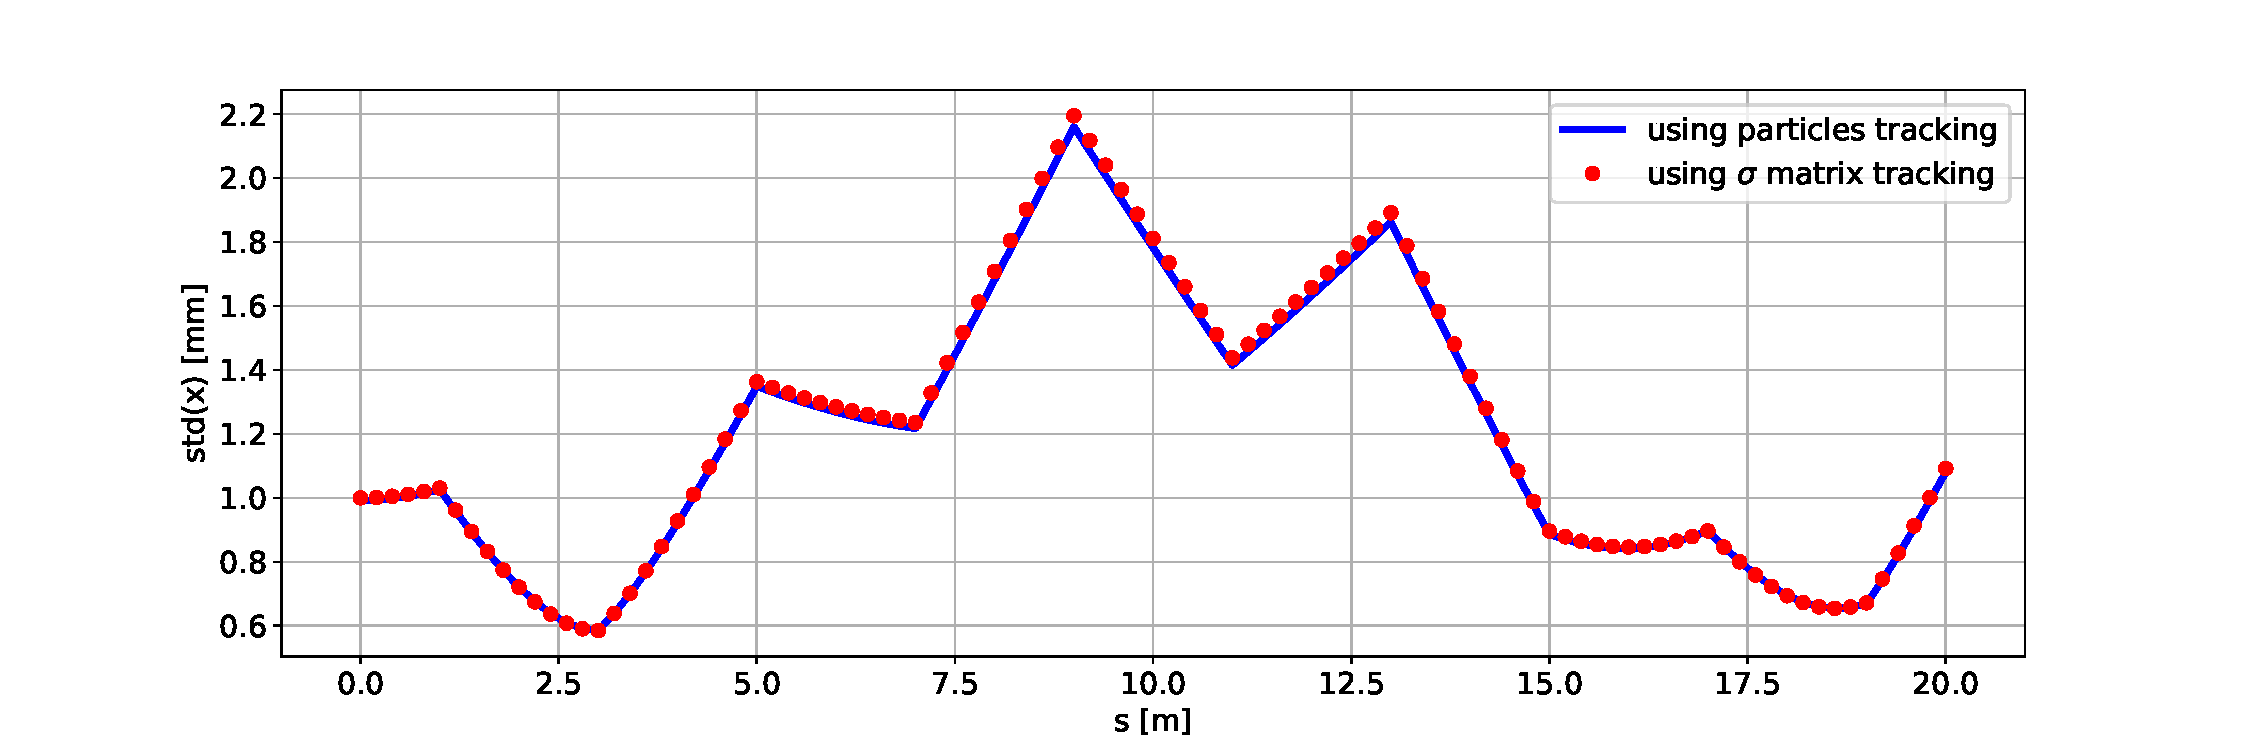
\includegraphics[width=\textwidth]{_img_primer/exercise_15.pdf}
\end{center}
\caption{\label{fig:sig2}The beam size (blue line) from Figure~\ref{fig:sigvzs} and calculated
  from Equation~\ref{eq:prop} (red markers).}
\end{figure}
%..............................................
The two equations in Equation~\ref{eq:prop} are particularly convenient and efficient to 
implement in software, because they just describe matrix multiplication of the centroid 
$\vec X$ and the sigma matrix $\sigma$, both of which describe the beam, and the transfer 
matrices $R,$ which describe the hardware of the beamline. We can now implement these
equations in the following code segment following code segment, where we add the calculations according to Equation~\ref{eq:prop}.
\begin{lstlisting}[language=Python]
#lattice
f = 2.5
L_2 = 2
fodo_lattice= 5*D(L_2/10) + Q(f) + 10*D(L_2/10) + Q(-f) + 5*D(L_2/10)

#prepare the beam
Npart = 10000
beam0 = np.random.randn(2, Npart)
x0 = 0;
xp0 = 1
sigx = 1; 
sigxp = 0.5/2; 
beam0[0,:] = sigx*beam0[0,:] + x0
beam0[1,:] = sigxp*beam0[1,:] + xp0

#prepare the sigma matrix
sigma0 = np.array([[sigx**2, 0], [0, sigxp**2]])
output_a = transportParticles(beam0, 5*fodo_lattice)


def transportSigmas(sigma, beamline):
    '''Transport the sigma matrix along the beamline'''
    coords = [sigma]
    s = [0]
    for elements in beamline:
        coords.append(elements['matrix'] @ coords[-1] @ elements['matrix'].transpose())
        s.append(s[-1] + elements['length']) 
    coords = np.array(coords).transpose()
    return {'sigma11': coords[0][0],
            'sigma12': coords[0][1],
            'sigma21': coords[1][0], # equal to sigma12
            'sigma22': coords[1][1],
            's':  np.array(s),
            'coords': coords,}

output_b = transportSigmas(sigma0, 5*fodo_lattice)

plt.plot(output_a['s'], np.std(output_a['x'],0), '-b', lw=3, label='using particles tracking')

plt.plot(output_b['s'], np.sqrt(output_b['sigma11']), 'or', lw=3, label='using $\sigma$ matrix tracking')
plt.grid(True)
plt.xlabel('s [m]')
plt.ylabel('std(x) [mm]')
plt.legend()
\end{lstlisting}
In this code segment, we adopt the same approach used for the {\tt beam0} vector to \texttt{sigma0}. We initialize the
{\tt sigma0} and then we loop
over the beamline element and propagate according to Equation~\ref{eq:prop}. 
Finally, we plot both the newly calculated beam sizes and those
calculated previously as a function of the $s$-position. The result, displayed in 
Figure~\ref{fig:sig2}, shows very good agreement of the beam sizes. Henceforth, we
will only use Equation~\ref{eq:prop} for propagating beams through beamlines.

\begin{exercise}
Using Equation~\ref{eq:prop}, display (a) the average position of the particles along the beamline. Likewise, (b) display the angular divergence. Compare with the result you found in Exercise~14.
\end{exercise}

In Figure~\ref{fig:sig2} the beam size $\sigma_x$ oscillates in a somewhat uncontrolled 
fashion along the beamline. Next we will explore whether we can find periodic oscillations
that repeat after each cell. 

\begin{exercise}
Can you find an initial beam matrix {\tt sigma0} that reproduces itself at the end of the beamline? \textbf{Hint}: proceed by try and error, you will see it is not trivial.
\end{exercise}


%
\section{Periodic systems and beams}
%
To explore the periodicity of a beam optical system, we first consider a single FODO
cell only and follow a single particle with initial coordinates $x=2$ mm and $x'=2$ mrad over 
a large number of turns, as shown in the following script. To speed up the computation (not strictly needed for this simple example) we ``compress'' the FODO lattice in a single transfer matrix (the so-called one-turn-map).
\begin{block}{Nota Bene}
The `one-turn-map' provide a very crucial insight of a closed machine (e.g., a synchrotron or a circular collider). In linear optics the one-turn-map is a matrix. By analyzing the matrix properties (e.g., eigenvalues decomposition) we can extract important stability and optics information.
\end{block}


The code used for the compression uses the {\tt getEquivalentElement} function. 
\begin{lstlisting}[language=Python]
f = 2.5
L_2 = 2
fodo_lattice = 5*D(L_2/10) + Q(f) + 10*D(L_2/10) + Q(-f) + 5*D(L_2/10)
OTM = getEquivalentElement(fodo_lattice)
particle = [[1],[.3]]
output = transportParticles(particle,100*OTM)

plt.plot(output['s']/(L_2*2), output['x'][0] ,'o-b')
plt.xlabel('Turns')
plt.ylabel('x [mm]')
plt.grid(True)
\end{lstlisting}

Once we got the one-turn-map we can track the particle following the usual approach. It the following code, we used also interactive plots to show the trace-space:
\begin{lstlisting}[language=Python]
from ipywidgets import interactive

f = -2.5
L_2 = 2
fodo_lattice = 5*D(L_2/10) + Q(-f) + 10*D(L_2/10) + Q(f) + 5*D(L_2/10)
OTM = getEquivalentElement(fodo_lattice)
def plotIt(x, xp):
    particle = [[x],[xp]]
    output = transportParticles(particle,100*OTM)
    plt.scatter(output['x'], output['px'], c = output['s']/(L_2*2))
    cb=plt.colorbar()
    cb.set_label('Turns')
    plt.xlabel('x [mm]')
    plt.ylabel("x' [mrad]")
    plt.xlim(-13,13)
    plt.ylim(-5,5)
    plt.grid(True)

interactive_plot = interactive(plotIt,x=(-2,2,.1),xp=(-2,2,.1),continuous_update=True)
output = interactive_plot.children[-1]
output.layout.height = '350px'
interactive_plot
\end{lstlisting}


%..............................................
\begin{figure}[tb]
\begin{center}
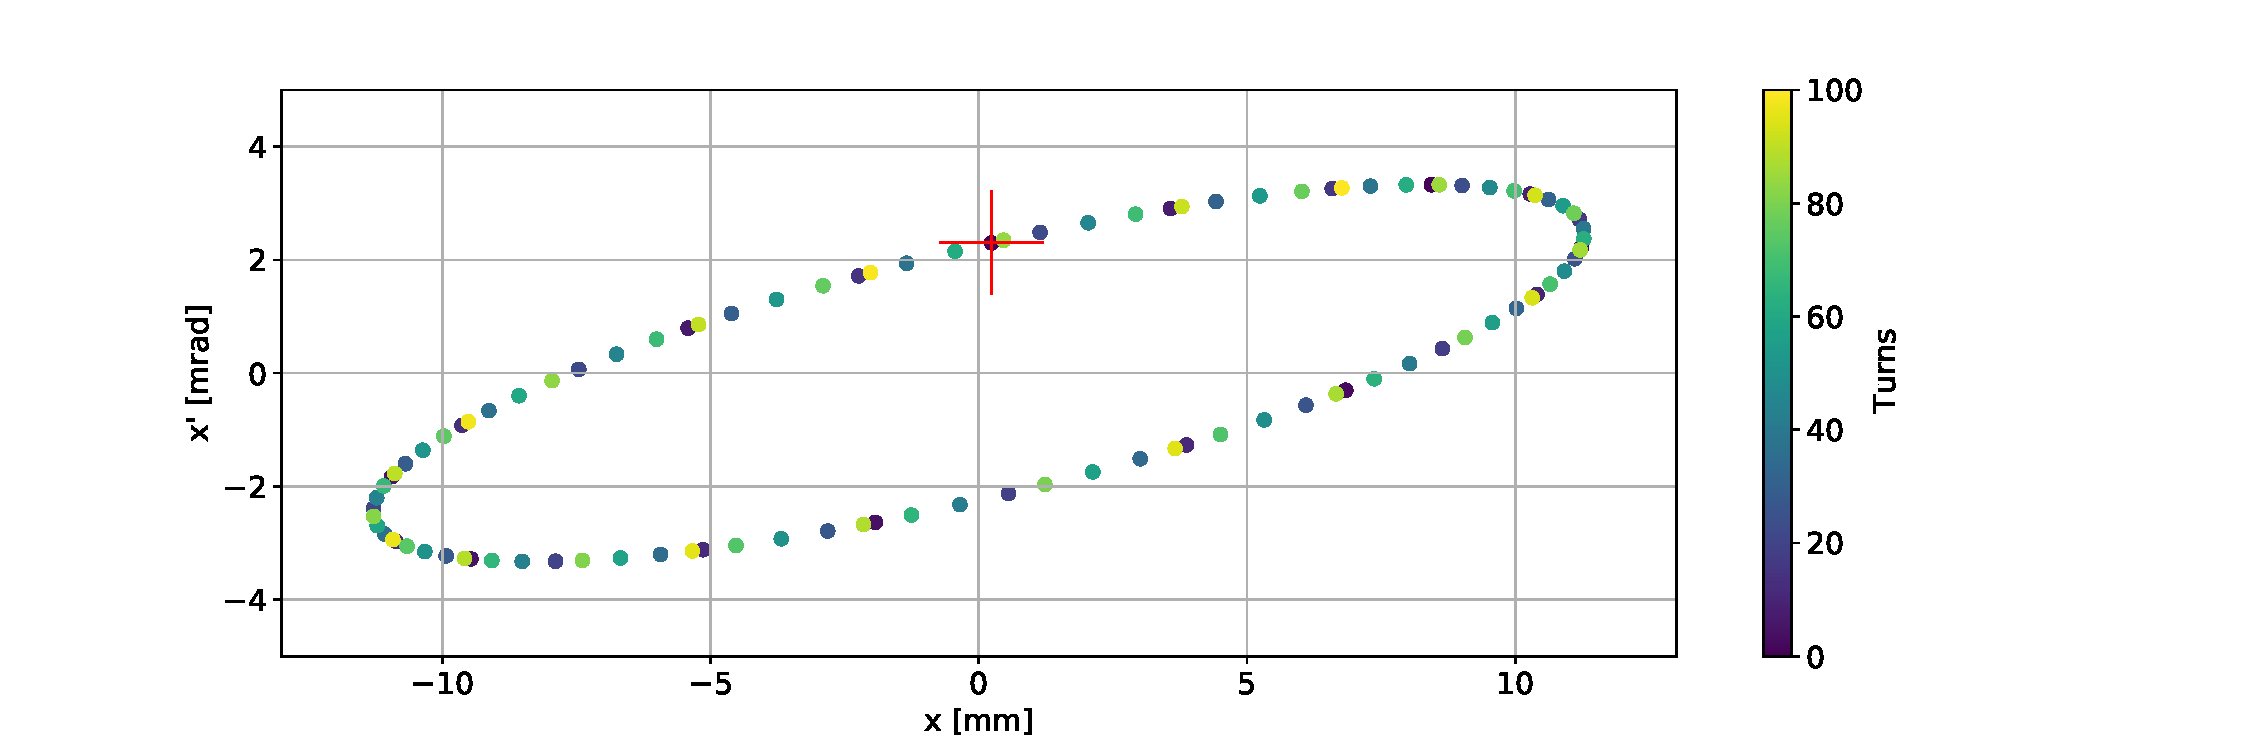
\includegraphics[width=1\textwidth]{_img_primer/exercise_18.pdf}
\end{center}
\caption{\label{fig:ps} A phase-space plot showing positions $x$ versus angles $x'$ of a particle followed for 100 consecutive turns. The red cross marker indicates the initial position of the particle.}
\end{figure}
%..............................................

The plot, shown in Figure~\ref{fig:ps},
displays an ellipse. 

\begin{exercise}
Explore different initial coordinate and compare the phase-space plots you obtain.
\end{exercise}

\begin{exercise}
Plot the x and x' for the different turns. What do you observe? 
  % (b) Execute {\tt plot(mod(spos,4),data(:,1),'*')} to display the
  % trajectory modulo the length of one FODO cell in order to see the trajectories that can
  % occur, all mapped into a single cell. What do you observe?
\end{exercise}
  
\begin{exercise}
In the definition of FODO of the previous exercise, reverse the polarity of both quadrupoles and prepare a phase-space plot. How does it differ from the one in Exercise~18?
\end{exercise}
  
\begin{exercise}
Prepare an array describing a FODO cell that starts immediately following the quadrupole with the negative focal length and prepare the phase-space plot. 
\end{exercise}

The particle, performing stable oscillations reminiscent of a harmonic oscillator, 
suggests that we can split the transfer matrix for one turn into a product of three 
matrices~\cite{VZAPB}; a rotation matrix, sandwiched between two matrices that distort 
the coordinates
\begin{equation}\label{eq:RAOR}
R={\cal A}^{-1}{\cal O}{\cal A}
\quad\mathrm{with}\quad
{\cal O}=\left(\begin{array}{rr} \cos\mu &\sin\mu\\ -\sin\mu & \cos\mu\end{array}\right)
\quad\mathrm{and}\quad
{\cal A}=
\left(\begin{array}{cc} \frac{1}{\sqrt{\beta}} & 0 \\ 
\frac{\alpha}{\sqrt{\beta}} & \sqrt{\beta}\end{array}\right)\, .
\end{equation}
Here $\alpha$ and $\beta$ are two, presently undetermined, parameters that describe the 
distortion. We can, however, determine them from $R$ by comparing coefficients with
the result 
\begin{equation}\label{eq:betaR}
\mu=\arccos\left(\frac{R_{11}+R_{22}}{2}\right)\ ,
\quad \beta=\frac{R_{12}}{\sin\mu}\ ,
\quad\mathrm{and}\quad \alpha=\frac{R_{11}-R_{22}}{2\sin\mu}\, .
\end{equation} 
These equations are encapsulated in the following function {\tt twiss}

\begin{lstlisting}[language=Python]
def twiss(beamline):
    '''Returns the Q, and the Twiss parameters beta, alpha, gamma of the beamline'''
    OTM = getEquivalentElement(beamline)
    R = OTM[0]['matrix']
    mu = np.arccos(0.5*(R[0,0]+R[1,1]))
    if (R[0,1]<0): 
        mu = 2*np.pi-mu;
    Q = mu/(2*np.pi)
    beta = R[0,1]/np.sin(mu)
    alpha = (0.5*(R[0,0]-R[1,1]))/np.sin(mu)
    gamma = (1+alpha**2)/beta
    return Q, beta, alpha, gamma
\end{lstlisting}
which allows us to determine the parameters $\alpha,\, \beta,$ and $\mu=2\pi Q$ from any
transfer matrix $R$ that permits stable oscillations. Note that this is only possible
for $\vert (R_{11}+R_{22})/2\vert <1,$ which indicates the limit of stability.

\begin{exercise}
Find the range of focal lengths {\tt F} for which the FODO cells permit stable oscillations.
\end{exercise}

The parameters returned by {\tt twiss} are commonly called the phase advance $\mu,$
the Twiss parameters $\alpha,\,\beta,$ and $\gamma=(1+\alpha^2)/\beta,$ and $Q$ is referred as the tune.
\par
So, why did we analyze the transfer matrix if we actually want to construct a 
sigma matrix that is periodic? Because the Twiss parameters make it particularly
simple to build a beam matrix {\tt sigma0} that repeats itself after one cell.
It is given by
\begin{equation}\label{eq:sigma0}
\sigma_0=\eps \left(\begin{array}{rr} \beta & -\alpha \\ -\alpha & \gamma \end{array}\right)\ ,
%=\eps {\cal A}^{-1} \left({\cal A}^{-1}\right)^t
\end{equation} 
where we introduced the emittance $\eps,$ whose relevance will become obvious in a short
while. We can now propagate the matrix $\sigma_0$ through the cell and use Equation~\ref{eq:RAOR} 
to express the transfer matrix $R$ through ${\cal A}$ and ${\cal O}.$ After some algebra, we
find
\begin{equation}
R\, \sigma_0\, R^t = \sigma_0\ ,
\end{equation}
which shows that the beam matrix, as defined in Equation~\ref{eq:sigma0}, reproduces itself 
after one cell. Let's try out whether this really works in the following code.

\begin{lstlisting}[language=Python]
f = 2.5
L_2 = 2
fodo_lattice = Q(2*f) + 10*D(L_2/10) + Q(-f) + 10*D(L_2/10) + Q(2*f)
OTM = getEquivalentElement(fodo_lattice)
tune, beta, alpha, gamma = twiss(OTM['matrix'])
sigma_0 = np.array([[beta, -alpha],[-alpha, gamma]])

def transportSigmas(sigma, beamline):
    '''Transport the sigma matrix along the beamline'''
    coords = [sigma]
    s = [0]
    for elements in beamline:
        coords.append(elements['matrix'] @ coords[-1] @ elements['matrix'].transpose())
        s.append(s[-1] + elements['length']) 
    coords = np.array(coords).transpose()
    return {'sigma11': coords[0][0],
            'sigma12': coords[0][1],
            'sigma21': coords[1][0], # equal to sigma12
            'sigma22': coords[1][1],
            's':  np.array(s),
            'coords': coords,}

output = transportSigmas(sigma_0, fodo_lattice)

plt.plot(output['s'],  output['sigma11'], '-b', lw=3, label='$\\beta_x\ [m]$')
plt.plot(output['s'], -output['sigma12'], '-r', lw=3, label='$\\alpha_x$')
    
plt.grid(True)
plt.legend(loc='best')

plt.xlabel('s [m]')
\end{lstlisting}
We also plot the $\beta$ and $\alpha$ function along the FODO lattice (Figure~\ref{fig:beta}).

%..............................................
\begin{figure}[tb]
\begin{center}
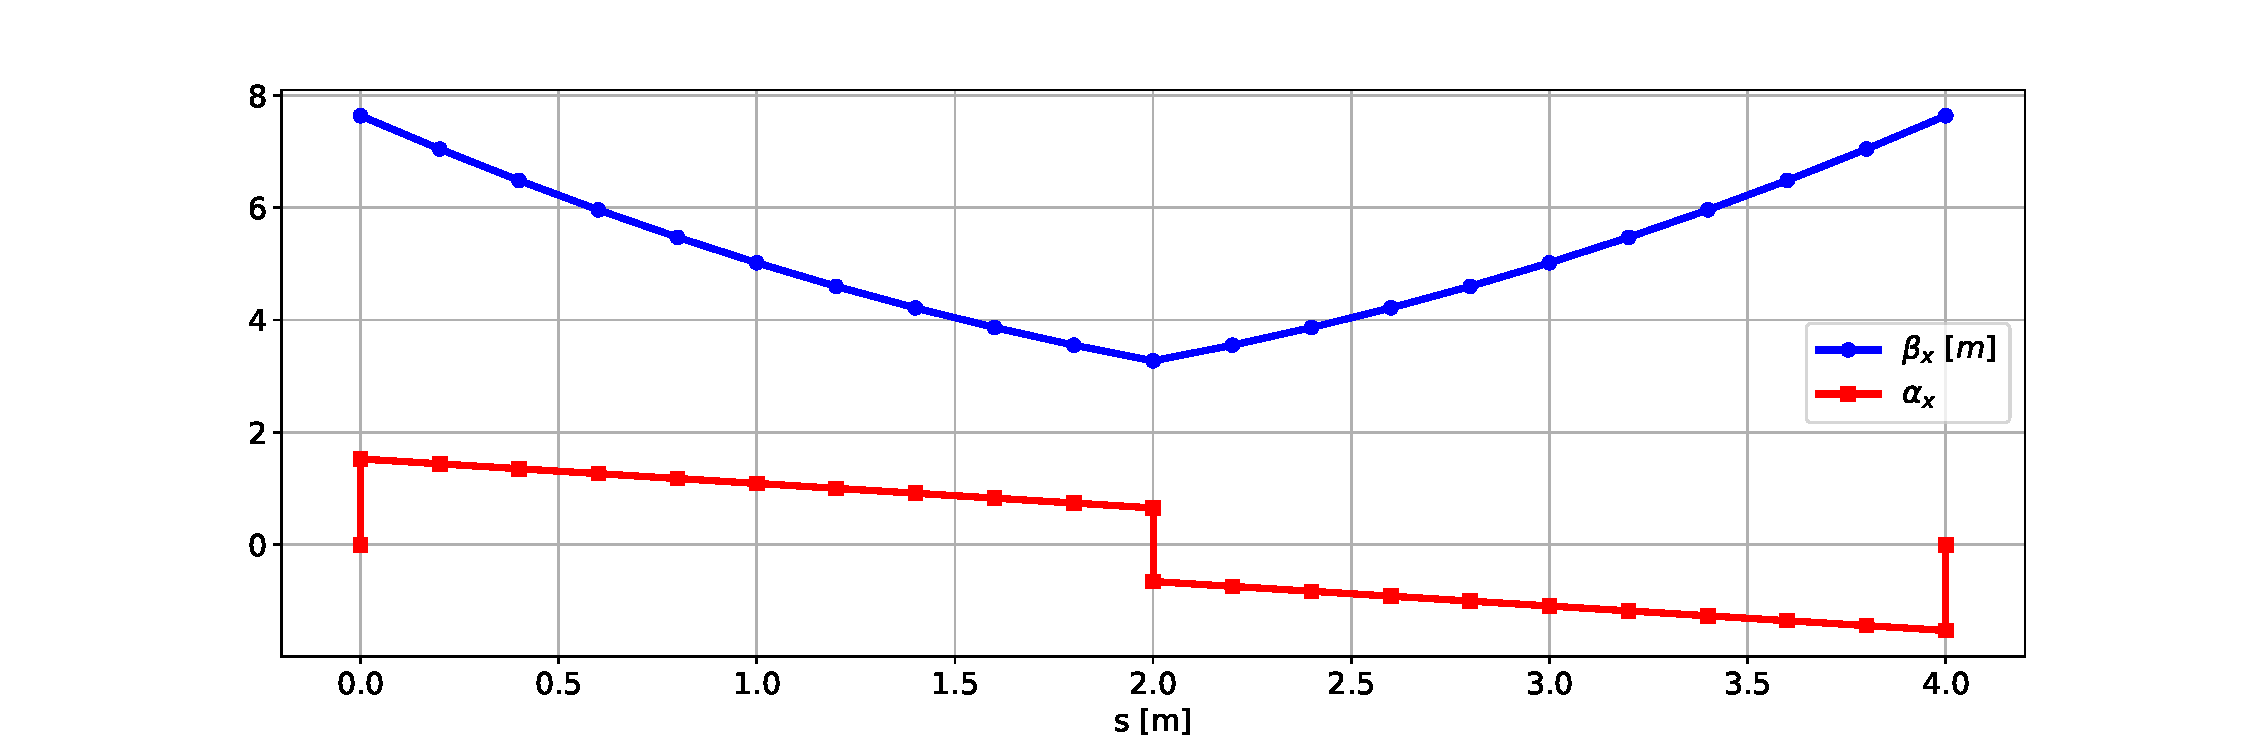
\includegraphics[width=1\textwidth]{_img_primer/exercise_23.pdf}
\end{center}
\caption{\label{fig:beta} Twiss parameters along the FODO cell.}
\end{figure}
%..............................................

\begin{exercise}
Transport the periodic $\sigma$ matrix along the FODO and convince yourself that the $\sigma$ matrix at the end of the FODO is indeed equal to the one at the start.
\end{exercise}

\begin{exercise}
Write down the numerical values of initial beam matrix {\tt sigma0}, then build a beamline made of 15 consecutive cells by changing the definition of {\tt beamline} and then, using {\tt sigma0} with the noted-down numbers, prepare a plot of the beam sizes along the 15 cells. Is it also periodic?
\end{exercise}

The emittance $\eps$ that appeared in Equation~\ref{eq:sigma0} as an arbitrary constant is
actually conserved when propagating the beam matrix, which is easily seen from 
\begin{equation}
\det(\sigma) = \det(\tilde R\, \sigma_0\, \tilde R^t) =
\det(\tilde R)\, \det(\sigma_0)\, \det(\tilde R^t) = \det(\sigma_0)=\eps^2
\end{equation}
for an arbitrary transfer matrix $\tilde R,$ because all transfer matrices have unit 
determinant. This is true for all maps that describe the motion of a beam through static
magnetic fields, in particular, for the matrices for drift space and quadrupole and 
therefore also for products of those elements. 

\begin{exercise}
Verify that the OTM has determinant equal to 1.
\end{exercise}

Note also that the matrix with the Twiss parameters $\alpha,\beta,$ and $\gamma,$ which
appears in Equation~\ref{eq:sigma0}, has
unit determinant by construction. The Twiss parameters $\alpha, \beta,$ and $\gamma$ 
describe the relative magnitude of the matrix elements in $\sigma_0$ and the
emittance $\eps$ determines the absolute magnitude of the beam. In particular, when
considering the $\sigma_{11}$ of a sigma matrix, we see that the absolute beam size is
given by $\sigma_x^2=\sigma_{11}=\eps\beta.$ Here the emittance $\eps$ is constant 
and sets the scale, whereas $\beta(s)$ describes the modulation of the beam size
along a beamline from one position $s$ to another.

\begin{exercise}
Multiply $\sigma_0$ from Exercise 24 by 17 and calculate the emittance. Then propagate the $\sigma$ matrix through the beamline from Exercise 24 and verify that the emittance of the sigma matrix after every element is indeed constant and equal to its initial value.
\end{exercise}

Up to now, we have used FODO cells and calculated the phase advance $\mu$ and the 
Twiss parameters from the transfer matrices. We now reverse the procedure and try
to find hardware parameters, such as the focal length of a quadrupole, to achieve
certain, desirable values. This procedure, commonly called {\em matching,} is the
topic of the next section.
%
\section{Satisfying one's desires: matching}
%
From the analysis of large circular accelerators it is known that an important parameter 
for the stability of periodically traversed beamlines is the phase advance $\mu$ of
a cell, or the tune $Q,$ which is the phase advance for the whole ring, 
divided by $2\pi.$ Let us consider a single cell first and try to adjust the
focal length {\tt f} of the quadrupoles to a value, such that the phase advance of
the cell is $\mu=60^\circ,$ which corresponds to $Q=\mu/2\pi=1/6.$ The following
short script first defines {\tt f} and {\tt fodo\_lattice}, then calls {\tt getEquivalentElement} to
calculate the transfer matrices, and finally uses it
as argument for {\tt twiss()}, which returns the phase advance and the Twiss 
parameters. 

\begin{lstlisting}[language=Python]
f = 2
L_2 = 2
fodo_lattice = Q(2*f) + 10*D(L_2/10) + Q(-f) + 10*D(L_2/10)+Q(2*f)
tune, beta, alpha, gamma = twiss(fodo_lattice)
print(f'The tune is {tune}.')
\end{lstlisting}

The 'print' statement serves only to display the value of {\tt Q} which is 
the sought-after phase advance $\mu$ divided by $2\pi.$

\begin{exercise}
Vary {\tt f} by hand and try to find (a) a value that returns $Q=1/6.$ (b) Then try to find a value of {\tt f} that produces a $90^\circ$ phase-advance. What is the corresponding value of $Q$?
\end{exercise}

This procedure mimics the matching done by the accelerator-design software. There
a optimizer minimizes a cost-function that encodes the desired constraints. In
Exercise~27 you have to do it by hand.
\par
A common task when designing accelerators is matching one section of a beamline
to another one. Here we will assume that the upstream beamline consists of
FODO cells with a $60^\circ$ phase advance and the downstream beamline of FODO cells 
with a $90^\circ$ phase advance. These are the cells with the focal length we calculated
in Exercise~27. In between the $60^\circ$ and $90^\circ,$ we place a third cell with two
quadrupoles that we will use to match the upstream to the downstream beamline.
To do so, we need to prepare periodic beam matrices {\tt sigma60} and
{\tt sigma90} for the respective sections. Note that {\tt sigma90} only depends 
on {\em two} parameters: the Twiss parameters $\alpha$ and $\beta,$ and therefore we 
also need {\em two} quadrupoles with independently variable focal length to adjust
until the final beam matrix equals {\tt sigma90}. See Figure~\ref{fig:matching}
for an illustration of the geometry.

\begin{exercise}
Implement the procedure described in the previous paragraph and match of a FODO lattice with $\mu=60^\circ$ and $\mu=90^\circ$.
\end{exercise}

The discussed matching tasks are only basic examples of the tasks encountered when
designing an accelerator. As mentioned before, most software packages have a 
more or less convenient way to specify the constraints to fulfill and the magnets
to vary to satisfy the constraints. Then the software automatically produces the
magnet settings. 
%..............................................
\begin{figure}[tb]
\begin{center}
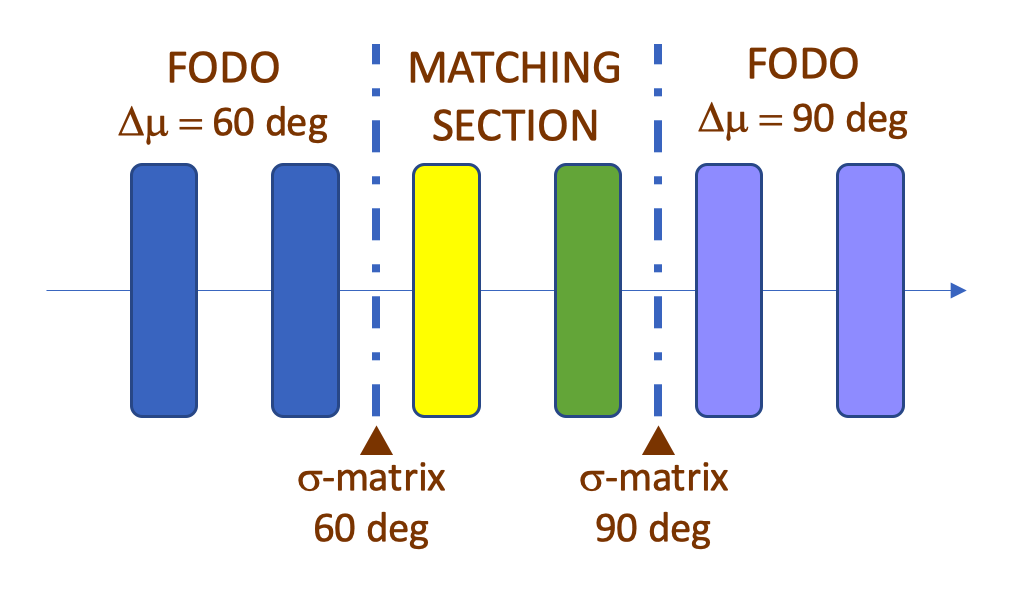
\includegraphics[width=.7\textwidth]{_img_primer/matching.png}
\end{center}
\caption{\label{fig:matching}Illustration for Exercise 28, where the strength of 
  the two matching quadrupoles needs to be determined.}
\end{figure}
%..............................................
%
%%%%%%%%%%%%%%%%%%%%%%%%%%%%%%%%%%%%%%%%%%%%%%%%%%%%%%%%%
%
\section{...and beyond...}
%
So far we only considered the very basic optical elements and confined ourselves to
a single transverse dimension. During CAS we will build on these basics and extend
the software in several directions. In this section, we therefore give some
indication of things to come. We start by including quadrupoles that have a finite
length. In the introductory beam optics lectures you will learn that the matrix for
these elements depends on the polarity of the magnet excitation, as specified by a
parameter $k_1\propto \pt B_y/\pt x.$ The matrix is given by
\begin{equation}\label{eq:QF}
Q(l,k_1)=\left(\begin{array}{cc}
\cos(\sqrt{k_1}l) & \frac{1}{\sqrt{k_1}}\sin(\sqrt{k_1}l) \\
-\sqrt{k_1}\sin(\sqrt{k_1}l) & \cos(\sqrt{k_1}l)\\
\end{array}\right)
\quad\mathrm{for}\quad k_1 \geq 0
\end{equation} 
and 
\begin{equation}\label{eq:QD}
Q(l,k_1)=\left(\begin{array}{cc}
\cosh(\sqrt{\vert k_1\vert}l) & \frac{1}{\sqrt{\vert k_1\vert}}\sinh(\sqrt{\vert k_1\vert}l) \\
\sqrt{\vert k_1\vert}\sinh(\sqrt{\vert k_1\vert}l) & \cosh(\sqrt{\vert k_1\vert}l)\\
\end{array}\right)
\quad\mathrm{for}\quad k_1 < 0
\end{equation}
and this brings us directly to 

\begin{exercise}
Introduce as a new element the thick quadrupoles matrices.
\textbf{Hint}:  write an external function that returns the corresponding list. 
\end{exercise}

Once the software is able to handle thick quadrupoles, we can replace the thin quadrupoles
in the beamline description used earlier.

\begin{exercise}
Use the beamline from Exercise~27 ($60^\circ$/cell FODO) and replace the thin quadrupoles by long quadrupoles with a length of 0.2, 0.4, 1.0\,m. Make sure the overall length and the phase advance of the FODO cell remains unchanged. By how much does the periodic beta function at the start of the cell change? Express the change in percent. 
\end{exercise}

In the introductory optics lectures you will learn that a so-called sector dipole magnet
will exhibit {\em weak focusing} in the bending plane. The transfer matrix for this 
magnet will be shown to be 
\begin{equation}\label{eq:BB}
B(l,\phi)=\left(\begin{array}{cc}
\cos(\phi) & \rho\sin(\phi) \\ -\sin(\phi)/\rho & \cos(\phi)
\end{array}\right)
\quad\mathrm{with}\quad \rho=l/\phi\, .
\end{equation}

\begin{exercise}
Implement in a Python function the element corresponding to the weak focusing of a sector bend.
\end{exercise}

\begin{exercise}
Insert 1\,m long dipoles in the center of the drift spaces of the FODO cells from Exercise~27 while keeping the length of the cell constant. Investigate deflection angles of $\phi=5^\circ,\, 10^\circ$ and $20^\circ$. Check by how much the periodic beta functions change. Why do they change? Explain. Can you compensate the phase advance $\mu$ by adjusting the strength or focal lengths of the quadrupoles?
\end{exercise}

All matrices discussed up to now only address one transverse plane and assume that all
particles have the same momentum $p_0$. 
\par
But this is only approximately true in a real 
accelerator and we therefore must take small momentum deviations $\delta = (p-p_0)/p_0$
into account. Instead of describing a particle by its transverse coordinates $(x,x')$
alone, we now characterize each particle by $(x,x',\delta),$ which requires to upgrade
the transfer matrices to $3\times 3$ matrices that operate on state vectors $(x,x',\delta).$
The matrix for a drift space therefore turns out to be
\begin{equation}
D(L)=\left(\begin{array}{ccc} 1 &L & 0\\ 0 & 1 & 0 \\ 0 & 0 & 1\end{array}\right)\, ,
\end{equation} 
with the original $2\times2$ matrix from Equation~\ref{eq:drift} in the top left corner,
a $1$ in the bottom right corner and zeros in the other positions of the third row and
the third column. The transfer matrices for thin and long quadrupoles are updated likewise.
Only the matrix for the sector dipole has non-zero entries in the third column
\begin{equation}
B(l,\phi)=
\left(\begin{array}{ccc}
\cos\phi & \rho\sin\phi      & \rho(1-\cos\phi) \\
-\sin(\phi)/\rho & \cos\phi  & \sin\phi \\
        0        &    0      & 1  \\
\end{array}\right)\, .
\end{equation}
In order not to mix functions with the same name, but using $3\times3$ instead of 
$2\times 2$ matrices, name the new elements conveniently or prepare a sub-directory for the upgraded functions.
\begin{exercise}
Upgrade the software to consistently handle $3\times3$ matrices for drift space, quadrupoles, and sector dipoles.
\end{exercise}
  
\begin{exercise}
Build a beamline of six FODO cells with a phase advance of $60^\circ$/cell (thin quadrupoles are OK to use) and add a sector bending magnet with length 1 m and bending angle $\phi=10^\circ$ in the center of each drift. You may have to play with the quadrupole values to make the phase advance close to $60^\circ$. But you probably already did this in Exercise~32.
\end{exercise}
  
\begin{exercise}
Use the starting conditions $(x_0,x_0',\delta)=(0,0,0)$ and plot the position along the beamline. Repeat this for $\delta=10^{-3}$ and for $\delta=3\times 10^{-3}$. Plot all three traces in the same graph. Discuss what you observe and explain.
\end{exercise}

We also need to upgrade the beam matrix $\sigma$ to be consistent with the 
$3\times 3$ transfer matrices. It is 
then a $3\times 3$ matrix itself with the original $2\times 2$ sigma-matrix from 
Equation~\ref{eq:bmat} in the top-left corner, zeros in the third column and row,
except the matrix element in the lower-right corner, which contains the square of
the momentum spread $\sigma_p.$ 

\begin{exercise}
Work out the transverse components of the periodic beam
  matrix $\sigma_0$. Assume that the emittance is $\eps_0=10^{-6}$\,meter-rad. 
  Furthermore, assume that the momentum spread $\sigma_{33}=\sigma_p^2$ is zero 
  and plot the beam size along the beamline.
\end{exercise}

\begin{exercise}
Plot the beam size for for $\sigma_p^2=10^{-3}$ and for $\sigma_p^2=3\times 10^{-3}$. What happens if you change the phase advance of the cell? Try out by slightly changing the focal lengths.
\end{exercise}

\begin{exercise}
Determine the periodic dispersion at the start of the cell. Then plot the dispersion in the cell. 
\end{exercise}

For these exercises you definitely need to consult the slides from the introductory
beam optics lectures for background information.
\par
Instead of adding the momentum deviation as additional degree of freedom for the 
simulation, we can extend the simulation to comprise of both transverse degrees
of freedom, the horizontal and the vertical plane. The matrices that describe
the dynamics are then $4\times4$ matrices with the matrices for the respective
planes filling the upper-left and the lower-right $2\times 2$ sub-matrices. As 
an illustration, we show the matrix for a focusing ($k_1>0$) quadrupole
\begin{equation}
Q(l,k_1)=\left(\begin{array}{cc} Q_F & 0_2 \\ 0_2 & Q_D \end{array}\right)\ ,
\end{equation} 
where $Q_F$ is the matrix from Equation~\ref{eq:QF}, $Q_D$ from Equation~\ref{eq:QD},
and $0_2$ is the $2\times2$ matrix containing only zeros. For $k_1<0$ the sub-matrices
$Q_F$ and $Q_D$ are exchanged. The matrix for a thin quadrupole is constructed likewise.
From the introductory lectures, we know that the matrix for sector dipole only shows
weak focusing in the horizontal plane, but behaves as a drift space in the vertical 
plane. Its matrix is therefore given by
\begin{equation}
B(l,\phi)= \left(\begin{array}{cc} B_2 & 0_2 \\ 0_2 & D_2 \end{array}\right)\ ,
\end{equation}
where $B_2$ is the $2\times 2$ matrix from Equation~\ref{eq:BB} and $D_2$ the matrix
for  a drift space from Equation~\ref{eq:drift}. Note that in this framework, we
assume that all particles have the reference momentum $p_0$ and we can therefore
ignore the momentum deviation~$\delta.$
\begin{exercise}
Convert the code to use $4\times4$ matrices, where the 
  third and fourth columns are associated with the vertical plane.  
\end{exercise}

Using this software to address the following exercises. Note that changing a quadrupole 
simultaneously affects the phases advances $\mu_x, \mu_y$ and the beta functions
in the respective planes.
\begin{exercise}
Start from a single FODO cell with $60^\circ$/cell you used 
  earlier. Insert sector bending magnets with a bending angle of $\phi=10^\circ$ in the 
  center of the drift spaces. The bending magnets will spoil the phase advance in 
  one plane. Now you have two phase advances and need to adjust both quadrupoles 
  (by hand to 2 significant figures) such that it really is $60^\circ$ in both planes. 
\end{exercise}  

\begin{exercise}  
Use the result from exercise 2 and adjust the two quadrupoles 
  such that the phase advance in the horizontal plane is 90 degrees, cell, while it 
  remains $60^\circ$/cell in the vertical plane. 
\end{exercise}  

\begin{exercise} 
Prepare a beamline with eight FODO cells without bending magnets
  and with $60^\circ$/cell phase advance in both planes. (a) Prepare the periodic beam 
  matrix {\tt sigma0} (4x4, uncoupled) as the initial beam and plot both beam sizes along the 
beamline. (b) Use {\tt sigma0} as the starting beam, but change the focal length of the 
  second quadrupole by 10\,\% and plot the beam sizes once again. Discuss your observations.
\end{exercise}  

\begin{exercise} 
From the lecture about betatron coupling identify the transfer 
  matrix for a solenoid and write a function that receives the longitudinal magnetic
  field $B_s$ and the length of the solenoid as input and returns the transfer matrix. 
  Then extend the simulation code to handle solenoids. Finally, define a beamline where 
  you place the solenoid in the middle of a FODO cell and follow a particle with initial 
  condition $(x_0,x'_0,y_0,y'_0)=(10^{-3}\,\mathrm{m},0,0,0).$ What do you observe? Is the motion 
  confined to the horizontal plane? 
\end{exercise}

And this brings us to the end of this tutorial. Here, we try to give some idea about
what goes on ``under the hood'' of full-blown beam optics codes, such as MAD-X~\cite{MADX}.
Moreover we hope to have provided some guidance on how to write such a simulation code 
yourself and how to use it to ``play around'' with simple beam-optical system and get 
a feeling for their behavior. But the story does not stop here. There are many more topic 
covered in the CERN Accelerator School and the more advanced 
textbooks~\cite{VZAPB,WOLSKI,WIEDEMANN,SYLEE}.
%
\bibliographystyle{plain}
\begin{thebibliography}{M}
%
\bibitem{PYTHON}
Python web site: \url{https://www.python.org}
%
\bibitem{OCTAVE}
Octave web site: \url{https://www.octave.org}
%
\bibitem{MATLAB}
MATLAB web site: \url{https://www.mathworks.com}

%
\bibitem{VZAPB}
V. Ziemann, {\em Hands-On Accelerator Physics Using MATLAB,} CRC Press, Boca Raton, 2019.
%
\bibitem{TUTOCT}
V. Ziemann, {\em Beam Optics Primer Using Octave or MATLAB},\\ 
\url{http://arxiv.org/abs/arXiv:1907.10987}.
%
\bibitem{SIEGMAN}
A. Siegman, {\em Lasers,} University Science Books, Sausalito, 1986.
%
\bibitem{WOLSKI}
A. Wolski, {\em Beam dynamics in high-energy particle accelerators,} Imperial College 
Press, London, 2014.
%
\bibitem{WIEDEMANN}
H. Wiedemann, {\em Particle Accelerator Physics (2 vol.),} Springer Verlag, Heidelberg, 1998.
%
\bibitem{SYLEE}
S.Y. Lee, {\em Accelerator Physics,} World Scientific, New Jersey, 2004
%
\bibitem{MADX}
MAD-X web site: \url{http://madx.web.cern.ch/madx/}
%
\bibitem{solutions}
G. Sterbini, A. Latina, V. Ziemann, {\em Solutions of the Exercises of the Transverse Linear Beam Dynamics Primer using Python}.
%
\end{thebibliography}
%
%%%%%%%%%%%%%%%%%%%%%%%%%%%%%%%%%%%%%%%%%%%%%%%%%%%%%%%%%%%%%%%%%%%%%%%
%
\appendix
%
\section{Propagating the moments of a distribution}
\label{sec:propmom}
%
Here we work out how the moments propagate through the beamline as a function
of the transfer matrix $R$ that maps particle coordinates from one place to another.
If we assume that the downstream coordinates $\hat x$ are given by $\vec{\hat x} = R\vec x$
with $\vec{\hat x}=(\hat x,\hat x')^t=(\hat x_1,\hat x_2)^t$, and the upstream 
coordinates by $\vec x=(x,x')^t=(x_1,x_2)^t.$ Note that here subscript $1$ labels 
the position and $2$ the angle. The equation that relates $\vec{\hat x}$ to $\vec x$ 
can then be written as $\hat x_i = \sum_{j=1}^2 R_{ij}x_j,$ which is valid for every particle
in the ensemble. We can therefore calculate the averages over the final distribution as
\begin{equation}\label{eq:xtransp}
\hat X_i = \langle \hat x_i\rangle = \langle \sum_{j=1}^2 R_{ij} x_j\rangle 
=  \sum_{j=1}^2 R_{ij}\langle x_j\rangle = \sum_{j=1}^2 R_{ij} X_j\ .
\end{equation}
Here the first equality is simply the definition of $\hat X_i$ and the second follows from
replacing the particle coordinates $\hat x_i$ through the transfer matrix elements $R_{ij}$ 
and the upstream coordinates $x_j.$ Since the same matrix $R$ applies to {\em all} particles,
we can pull it out of the averaging, likewise with the summation over $j.$ But then we are 
left with the averages of $\langle x_j\rangle,$ which is the same as $X_j.$ This simple 
calculation proves the remarkable fact that the {\em beam centroids propagate in the same 
way as individual particles} and we can visualize the beam centroid as some sort of
super-particle. Note, however, that this feature depends crucially that the propagation
is described by a linear operation --- a matrix multiplication. If non-linear elements, such
as sextupoles are present in the beamline, this correspondence is no longer strictly true.
\par
Now we consider the second moments, but assume that the centroids are zero $X_i=0,$ which
simplifies the notation. The sigma-matrix elements $\hat\sigma_{ij}$ ``on the other end of 
the transfer matrix $R$'' can be calculated in the following way
\begin{equation}\label{eq:sigma1}
\hat\sigma_{ij} 
  =  \langle \sum_{k=1}^2 R_{ik}\, x_k \sum_{l=1}^2 R_{jl}\, x_l \rangle
  =   \sum_{k=1}^2 R_{ik}  \sum_{l=1}^2 R_{jl}\, \langle x_k x_l \rangle
  =  \sum_{k=1}^2\sum_{l=1}^2 R_{ik} R_{jl}\, \sigma_{kl}\, ,
\end{equation}
where the first equality follows from inserting $\hat x_i=\sum_{j=1}^2 R_{ij}\, x_j$ in the
definition of $\hat\sigma_{ij}= \langle \hat x_i \hat x_j \rangle$. Since the transfer 
matrices are constant and summing is linear, we can extract both sum and $R$ from the
averaging, denoted by the angle brackets and find that the sigma matrix transform 
according to
\begin{equation}\label{eq:sigma}
\hat\sigma = R\, \sigma\, R^t\, ,
\end{equation}
where we converted the expression from Equation~\ref{eq:sigma1}, which is given in 
components, into a matrix equation. Note that $R^t$ denotes the transpose of the matrix 
$R.$ Equations~\ref{eq:xtransp} and~\ref{eq:sigma} are given in Equation~\ref{eq:prop}
in Section~5 in the main part of the text.
\end{document}


% Davide Aug 2022 - place holder for possible additional exercise on emittance
\section{On the emittance definition}
\label{sec:emittance}
The motion of a single particle in the $x-x'$ phase space at the location $s$ is described using the Courant-Snyder parameters, $(\beta_s, \gamma_s, \alpha_s)$ as in \cite{book:edwards}:
\begin{equation}
\frac{\epsilon}{\pi} = \gamma_s x_s^2 + 2 \alpha_s x_s x'_s + \beta_s x_s'^2 \label{eq:ellipe}
\end{equation}
and where $\epsilon$ is the area enclosed by the ellipse defined by Eq.~\ref{eq:ellipe}.
Using this definition, the fraction $F$ of particles of a Gaussian-distributed beam that fall within the area defined above is:
\begin{equation}
    \epsilon = - \frac{2 \pi \sigma^2}{\beta_s} \ln(1-F)
\end{equation}
The area enclosing 95\% of the particles is:
\begin{equation}
    \epsilon = 6 \pi \sigma_s^2 / \beta_s
\end{equation}
where $\sigma_s$ is the rms transverse beam size.
The $x_{\text{max}}$ is
\begin{equation}
x_{\text{max}} \sqrt{\frac{\epsilon \beta_s}{\pi}}
\end{equation}
where $\epsilon$ choice depends on the number of particles to be included in the corresponding phase-space area.

\bibitem{book:edwards} Edwards, D. A., Syphers, M. J., ``An introduction to the physics of high energy accelerators,'' New York: Wiley. ISBN 978-0-471-55163--8, 1993.

\end{document}